%!TEX root = ../template.tex
%%%%%%%%%%%%%%%%%%%%%%%%%%%%%%%%%%%%%%%%%%%%%%%%%%%%%%%%%%%%%%%%%%%%
%% chapter4.tex
%% NOVA thesis document file
%%
%% Chapter with lots of dummy text
%%%%%%%%%%%%%%%%%%%%%%%%%%%%%%%%%%%%%%%%%%%%%%%%%%%%%%%%%%%%%%%%%%%%

\typeout{NT FILE chapter4.tex}%
\chapter{System Design and Implementation}
\label{cha:system_implementation}
This chapter begins with an introduction to the technologies used for the implementation in Section \ref{sec:tools}.
Subsequently, the overall architecture is followed by a support diagram, in Section \ref{sec:architecture}.
In Section \ref{sec:implementation}, all the implementation processes and features are developed.
Section \ref{sec:database} includes the data management and structured design.
Finally, the Section \ref{sec:design} explains the design path followed.

\section{Adopted Tools and Tecnhologies}
\label{sec:tools}
The following section focuses on the technologies and tools used in implementing this project. 
These include environments used, Unity, development tools, backend, database, and plugins.

\subsection{Working Environment}

The  \gls{VR} environment was developed using the Unity editor, with code scripts written in C\# within the \textbf{Visual Studio Integrated Development Environment (IDE)}.
Its features, such as debugging tools, error detection, code navigation, Unity-specific types recognized automatically, and IntelliSense suggestions, greatly enhanced productivity. 
To further support this integration, the Visual Studio Editor package was utilized. 

For the backend implementation, comprising the Node.js server and the database, \textbf{Visual Studio Code (VSCode)} was utilized. 
The same IDE was also adopted for the report writing in LaTeX, due to Overleaf limitations.

The version control system used initially for project management was \textbf{GitHub}, providing effective tracking of updates and overall code organization.
However, as a consequence of storage limitations in handling large files, such as the \gls{2D} ground view or the funerary enclosure \gls{3D} model, the \textbf{Diversion} tool was employed as an alternative solution for managing these system.

\subsection{Unity}
\textbf{Unity} is a cross-platform engine that provides a robust environment for developing \gls{2D} and \gls{3D} applications. 
Its component-based architecture simplifies \gls{3D} development by allowing developers to define object behaviors through scripts in \glspl{VE}.
Unity also offers a community forum and repositories available in \textbf{Unity Asset Store}\footnote{\url{https://assetstore.unity.com/}} where developers can access resources and adapt them for their projects.

For this study, Unity was selected for developing the \gls{VR} environment. The C\# programming language within Unity facilitates the management of game objects and user interactions in the \gls{VE}.
Its integration enables users an immersive experience while interacting with \gls{UI}, using the \gls{HMD}. 
The headset device used for testing during the implementation and for user evaluation was \textbf{Meta Quest 3}.

The following packages of Unity Asset Store were used to enhance the \gls{UI} and streamline the development process:

\begin{itemize}
\item{\textbf{Free UI Click Sound Pack}\footnote{\url{https://assetstore.unity.com/packages/audio/sound-fx/free-ui-click-sound-pack-244644}} - This package provides a collection of diverse clickable sounds, designed to provide an immersive and complete \gls{UX}.}
\item{\textbf{Simple Pie Menu}\footnote{\url{https://assetstore.unity.com/packages/tools/gui/simple-pie-menu-radial-menu-asset-270056}}} - A radial menu system implemented as the main menu of the project. Further details on its functionality are provided in Section \ref{sec:main_menu}.
\item{\textbf{White \& Black GUI}\footnote{\url{https://assetstore.unity.com/packages/2d/gui/icons/white-black-gui-by-gamertose-168805}}} - This package includes a range of trivial and useful icons used to guide users in navigating menu items and to support image gallery switching between pre- and post-intervention object states.
\end{itemize}

%Additionally, the \textbf{Unity Learn}\footnote{\url{https://learn.unity.com/}} platform provided free tutorials, substantially simplifying the learning process during development.

\subsection{Tools}
\textbf{Blender} is an open-source computer graphics software useful to a wide range of tasks, such as model, animate, create textures, materials. 
This tool was used to create an aproximation of the original texture of the glass object. Originally transparent, translucent.

\textbf{GIMP}, an open-source cross-platform image editor, was used to edit the map draw for integration as ground in Unity (rotated and cropped).
Additionally, GIMP was useful in editing the post-intervention object images. The object's images were cut out from their backgrounds, which were then replaced with a neutral grey. 
This enhanced clarity for users and allowed easy comparison between the object's before and after the cleaning and conservation treatment.

\subsubsection{Photogrammetry}
\label{sec:photogrammetry_tool} 

The software used to process digital images and generate the \gls{3D} model of the funerary enclosure was \textit{Agisoft Metashape}\footnote{\url{https://www.agisoft.com/}}.
This software performs photogrammetric processing of digital images to generate \gls{3D} spatial data, which can be applied in various fields such as \gls{GIS} applications, \gls{CH} documentation, visual effects production, and indirect measurements of objects of diverse scales. 

 A total of 143 images were collected after the excavation campaign by the archaeologist responsible for thIS site.
 % by the restoration department of NOVA for analysis. 
Based on these images, a \gls{3D} model of the funerary enclosure was generated, as described in Section \ref{sec:build_model}.
Two already built models of artefacts were provided by Sofia Pires.

\subsection{Backend \& Data Management}
This section includes the backend and database repository technologies choices. 
\subsubsection{Backend}

The backend technology selected for this thesis was \textbf{Node.js}, an open-source, cross-platform JavaScript runtime environment. 
Node.js enables developers to create servers, web applications, command-line tools, and automation programs.

In this thesis, Node.js was used to support the web server and to improve performance and scalability when handling repository data. 
Additionally, it will streamline the communication between Unity and the database repository.

Express.js is the most popular Node.js web application framework, widely used for building web applications and \gls{API}s, with a minimal and flexible design.
In this study, the web server Express.js\footnote{\url{https://expressjs.com/}} was used to expose the REST endpoints.


\subsubsection{Database Repository}
\label{sec:repos}

There are several alternatives for storage management systems, but the option shelt for this project was \textbf{PostgreSQL} for its geographical extension, PostGIS, and its relational database is more appropriate due to its flexibility and consistency.
Additionally, because of its high performance and flexibility in managing spatial data. 

PostGIS is widely used for spatial data storage, geometry processing, and efficient geospatial querying.

\subsection{XR Components and Plugins}
This section comprises the main plugins and components used to support the custom implementation.
\subsubsection{XR Plugin Management}
The \textbf{XR Plugin Management} package was used to simplify the integration and management of various XR plug-ins. 
This package is primarily responsible for loading, initializing, configuring settings, and providing build support for XR features. 
It was used in conjunction with the OpenXR.

\textbf{OpenXR} is an open-standard \gls{API} enabling cross-platform development, with a high-performance access to AR and VR paltforms and devices. In this sudy this plugin, handles communication with the \gls{VR} headset.

\subsubsection{XR Interaction Toolkit}
The \textbf{XR Interaction Toolkit} was a central component in the development process, providing essential interaction capabilities and abstracting much of the low-level complexity of \gls{VR} development. It enabled features such as Hand tracking, 
Object interaction (e.g., grab and release), Teleportation-based locomotion, \gls{UI} interaction, and Controller support.

\subsubsection{User Movement Components}
The \textbf{XR Origin} served as the root GameObject that encapsulates the main camera and controller setup. 
It handles camera tracking based on the user's head movement and manages controller positioning and orientation. 
Within this structure, the XR Rig was used as the container for the camera and associated controllers.

To implement user movement within the \gls{VE}, the Locomotion System package was utilized. The following components were integrated: 

\begin{itemize}
\item{\textbf{Continuous Move Provider:}  Allowed smooth movement via the right joystick.}
\item{\textbf{Snap Turn Provider:}  Enabled rotational movement in fixed increments, chosen over continuous turning to reduce motion sickness.}
\item{\textbf{Teleportation Provider:} Enabled teleportation across the plane surface using the left joystick.}
\item{\textbf{Teleportation Anchors:} Defined specific teleportation points, represented as buttons.}
\end{itemize}

\subsubsection{User Interaction Components}
For interaction within the virtual scene, the toolkit offered components such as the XR Near-far interactor, that provided a way to interact with the scene through the ray emitted from the controllers, and the XR Grab Interactable enabled direct manipulation of virtual objects through grabbing, holding, and releasing actions.

For input handling, Unity provides two systems: the old Input Manager and the newer \textbf{Input System Package}. 
While the Input Manager is built into the Unity engine and used by default, the project adopted the Input System Package due to its flexibility, and scalability. 
This newer system supports a wide range of input devices and enables precise configuration through a centralized interface. Input actions are defined and managed using the Input Action Manager, which allows the developer to specify actions and map them to devices or controls. 
Each input action is activated as needed during runtime, offering an adaptable input handling framework.


\section{System Architecture}
\label{sec:architecture}

The system is divided into three application layers.
The \textbf{Presentation Layer} manages the \gls{VR} environment and its interaction with users. The \textbf{Application Layer} includes the management of Unity Requests, with the support of the framework "UnityWebRequest" REF, acting as an intermediate between the Unity client and the database. 
The communication flow between these layers is managed through a Node.js REST API, chosen for its flexibility and lightweight design. 
Finally, the \textbf{Data Access Layer} contains the database, which stores all information related to object data, excavation, and object interventions. 
The architecture of the system can be observed in Figure \ref{fig:architecture}.
\begin{figure}[h!]
    \centering
    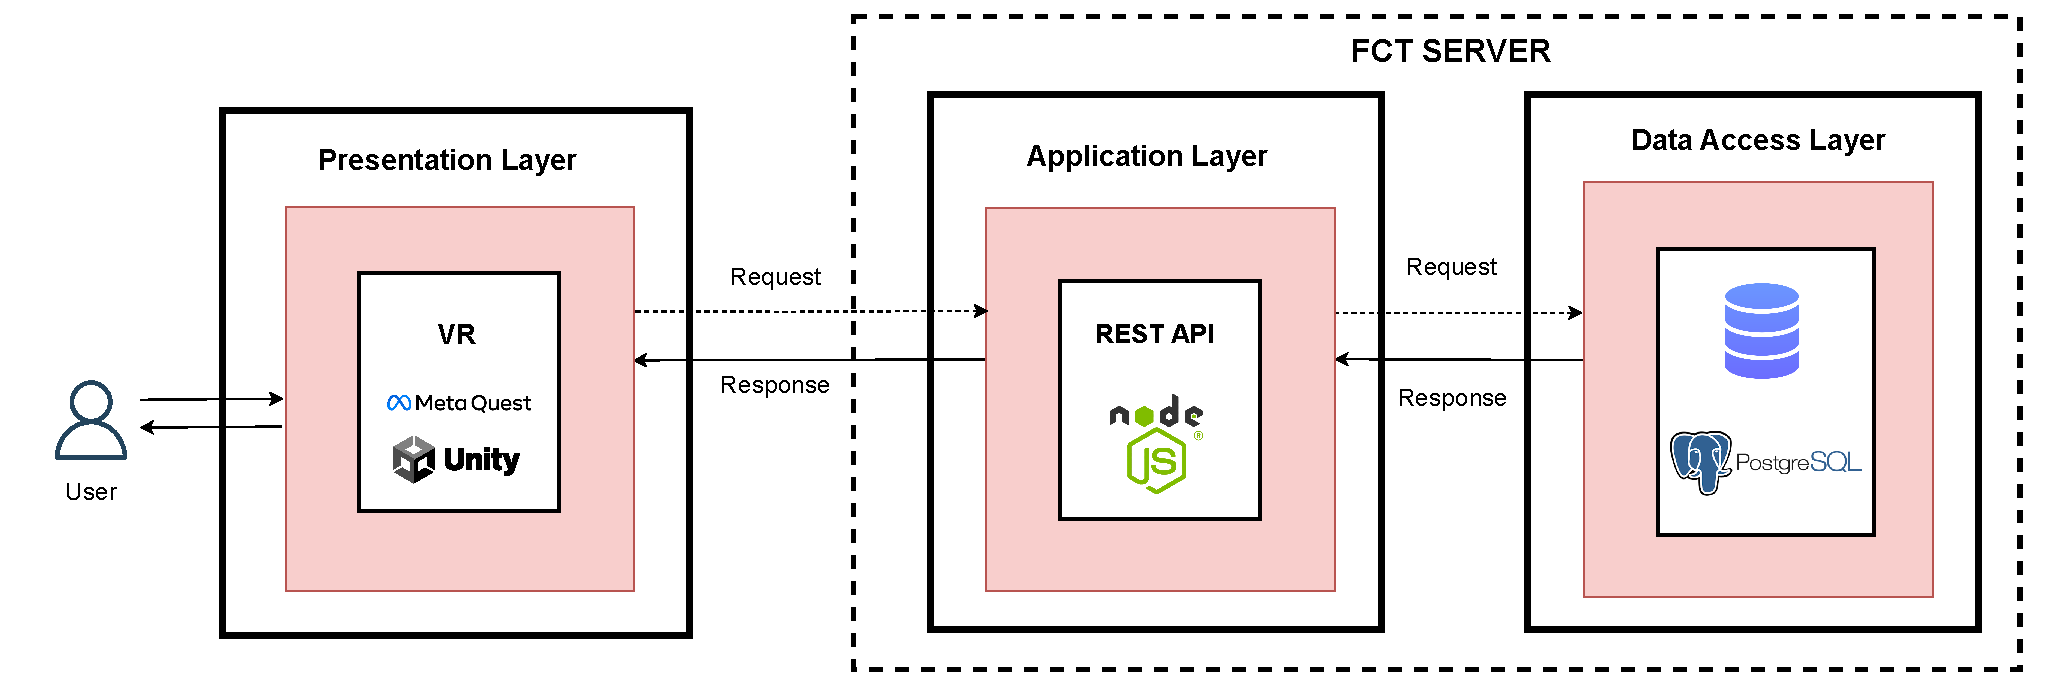
\includegraphics[width=1\linewidth]{Diagrama_Arquitetura}
    \caption{System Architecture Overview of the Developed System. \textcopyright\ Ana Maissa Antunes}
    \label{fig:architecture}
\end{figure}

During the development stage, the database was hosted locally on a PostgreSQL server managed via pgAdmin\footnote{\url{https://www.pgadmin.org/}}, an Open Source management tool for PostgreSQL. To access and present data in Unity, it was necessary to manually execute the "index.js" file, which contained the Node.js API endpoints.
Subsequently, before the user testing phase, the backend code, comprising both the API endpoints and the PostgreSQL database, was deployed to the \gls{FCT} Server with a dedicated service.
This deployment ensured that the server hosting the API endpoints remained continuously active, allowing Unity clients to retrieve data seamlessly without manual intervention.

\section{System Implementation}
\label{sec:implementation}

This section starts with some explanation of the implementation scripts made from Unity to the Database.
After that, it contains the implementation process of all functionalities developed within the \gls{VE}.
The following is the method explanation of the three fundamental techniques.
Finally, testing and debugging methodologies were applied during the dissertation.

\subsection{Communication between Unity and Database}

The \textbf{UnityWebRequest} class is used to send HTTP requests to the Node.js server, supporting both options retrieval (Section \ref{sec:options}) and object data retrieval (Section \ref{sec:data_retrieval}).

The structures required to retrieve the desired object attributes are represented in Listing \ref{lst:structure}.

\begin{lstlisting}[language=C++, caption={Artifact Structure to extract responses.}, label={lst:structure}]
public class Dimensions
{
    public float height;
    public float width;
    public float weight;
}

public class Artifact
{
    public int id;
    public int tomb_id;
    public string name;
    public string material;
    public string glass_type;
    public string shape;
    public Dimensions dimensions;
    public bool is_fragmented;
    public bool has_pontil_mark;
    public bool has_gold_fragments;
    public string provenance;
    public string general_description;
    public string epoch;
    public string[] paralels_url;
    public string[] images_path_b_interv;
    public string[] images_path_a_interv;
}
public class ArtifactList
{
    public List<Artifact> items;
}
\end{lstlisting}

\subsubsection{Dropdown Options Retrieval}
\label{sec:options}
The request is sent to the \textbf{/GET (get-objects\_data)} endpoint, with the \texttt{url} as a parameter.
The artifacts returned from the database are wrapped into a list structure, which is then iterated to add each ID to the dropdown \texttt{options} list, as shown in Listing \ref{lst:artifact_ids}.

\begin{lstlisting}[language=C++, caption={Method used to load artifact IDs and define as options in the Dropdown.}, label={lst:artifact_ids}]
      IEnumerator GetOptionsIds(string url)
    {
        UnityWebRequest www = UnityWebRequest.Get(url);
        ...
        if (www.result == UnityWebRequest.Result.Success)
        {
            ...
            ArtifactList artifactList = JsonUtility.FromJson<ArtifactList>(wrappedJson);
            
            List<TMP_Dropdown.OptionData> options = new List<TMP_Dropdown.OptionData>();
            ...
            foreach (Artifact artifact in artifactList.items)
            {
                string id = artifact.id.ToString();
                options.Add(new TMP_Dropdown.OptionData("     " + id));
            }
            dropdown.AddOptions(options);
        }
        else{
            Debug.LogError("Error: " + www.error);
        }
    }
\end{lstlisting}


\subsubsection{Object Data Retrieval}
\label{sec:data_retrieval}
This method, shown in Listing \ref{lst:get_data}, retrieves all data of objects necessary to present in the \gls{VE}.  
It sends a \texttt{GET} request to obtain the complete information, including images before and after intervention, which are then passed to \texttt{GetImages()}, explained in the section below.  

Additionally, textual data is retrieved. Once the request is successful, the JSON response is parsed into an \texttt{Artifact} object using Unity's \texttt{JsonUtility.FromJson<Artifact>()} method.  
From this structure, the following relevant fields are extracted: \emph{id}, \emph{name}, \emph{material}, \emph{epoch}, \emph{provenance}, and \emph{dimensions}.  
The \emph{dimensions} field is a nested JSON structure containing \emph{height}, \emph{width}, and \emph{weight}.  

Finally, a formatted string is created to display the object's details in the \gls{UI} panel.

\begin{lstlisting}[language=C++,label={lst:get_data}, caption={Method used to get object data from the database doing.}]
      IEnumerator GetData(string url)
    {
        UnityWebRequest www = UnityWebRequest.Get(url);
        yield return www.SendWebRequest();

        if (www.result == UnityWebRequest.Result.Success)
        {
             artifact = JsonUtility.FromJson<Artifact>(www.downloadHandler.text);

            string displayText = "<b>Object Details:</b>\n\n";

            string material = artifact.material.Replace("{", "").Replace("}", "");

             displayText += $"ID: {artifact.id} | Name: {artifact.name} \nMaterial: {material} | Epoch: {artifact.epoch} \nProvenance: {artifact.provenance}" +
                         $"\nDimensions: {artifact.dimensions.height} x {artifact.dimensions.width} cm, Weight: {Mathf.Round(artifact.dimensions.weight * 10.0f) * 0.1f} g";

            resultText.text = displayText;

            GetImages(artifact.id, artifact.images_path_b_interv);
        }
        ...
    }
\end{lstlisting}

\subsubsection{Object Images Retrieval}

The \texttt{GetImages} method iterates over the array of image paths retrieved from the "object\_intervention" table. The array passed to this method may be either "images\_path\_b\_interv", containing the object images before intervention, or "images\_path\_a\_interv", after the intervention.
For each image, a component is created and positioned appropriately within the gallery.

The implementation of this process is presented in Listing \ref{lst:artifact_images}.

\begin{lstlisting}[language=C++, caption={Method used to load artifact images and to display them in the Images Gallery.}, label={lst:artifact_images}]
      private void GetImages(int id, string[] images_path)
    {
        if (images_path.Length != 0)
        {
            changeView.SetActive(true);

            for (int x = 0; x < images_path.Length; x++)
            {
                var imagePath = images_path[x];

                if (x > images_path.Length / 2) {height = 0;}
                else if (x == images_path.Length / 2) { x_pos = 1.5f; height = 0; }
                else { height = 1; }

                Sprite sprite = Resources.Load<Sprite>("Images/" + imagePath);
                if (sprite != null)
                {
                    GameObject newImgObj = new GameObject("Image_" + imagePath, typeof(RectTransform), typeof(CanvasRenderer), typeof(Image));
                    newImgObj.transform.SetParent(imageParent, false);

                    RectTransform rectTransform = newImgObj.GetComponent<RectTransform>();
                    rectTransform.sizeDelta = new Vector2(1, 1);
                    rectTransform.localPosition = new Vector3(x_pos++, height, 0);

                    Image imgComponent = newImgObj.GetComponent<Image>();
                    imgComponent.sprite = sprite;
                }
                ...
            }
            x_pos = 1.5f;
        }
        else
        {
            Debug.LogWarning("Couldn't load Images for Object ID" + id);
        }
    }
\end{lstlisting}


\subsubsection{API Endpoints}

To retrieve information for each object, requests are made to the repository layer. 
Two main API endpoints were implemented for this purpose:

\begin{enumerate}
  \item \textbf{/GET (get-objects\_data)}
  \\Retrieves a list of object IDs by querying the \textbf{"object"} table. These IDs are used to populate the dropdown menu options in the \gls{UI}.

  \item \textbf{/GET (get-objects\_data/:id)}
  \\Fetches detailed information for a specific object based on its ID. This request is triggered when a user selects an object ID from the dropdown menu in the \gls{UI}
  Whenever the ID in the dropdown is changed, the system issues a new request for the corresponding ID, and the visualization panel and image gallery are updated accordingly.

  The representation of this endpoint is shown in Listing \ref{lst:api}. As illustrated int line 5, the query joins two tables, \textbf{"object"} and \textbf{"object\_intervention"}, to fetch simultaneously object data and images before and after interventions for display in the Image Gallery, described in Section \ref{sec:image_gallery}. 
  This SQL query enables the system to retrieve all necessary information with a single request after the user selects an object ID, thereby improving efficiency and reducing the need for multiple requests.

\end{enumerate}

\begin{lstlisting}[language=C++, caption={Example of defining an API endpoint in Node.js.},label={lst:api}]
  app.get('/get-objects_data/:id', async (req, res) => {
    const id = req.params.id;

    try {
        const result = await pool.query('SELECT * FROM object inner join object_intervention on object.id = object_intervention.object_id WHERE object.id = $1', [id]);
        res.json(result.rows[0]);
    } catch (error) {
        console.error(error);
        res.status(500).send('Server Error');
    }
});
\end{lstlisting}


\subsection{Virtual Environment}
The initial step was to place the \gls{2D} map on the ground plane, using the 1-meter default grid scale of Unity to ensure the precise real-world dimensions. With this in place, it was only necessary to adjust the scale of the funerary enclosure to match its position on the map. It is also important to mention that the two objects in the environment were carefully measured using virtual rules.

In the \gls{VE}, a set of functionalities was implemented. 
They are described in this section, in the following order: the Main Menu in Section \ref{sec:main_menu}, the Panel \gls{UI} in Section \ref{sec:panel_UI}, the Image Gallery in Section \ref{sec:image_gallery}, object interaction starting with the Slider in Section \ref{sec:object_slider}, the Outline in Section \ref{sec:object_outline}, and Grab and Release in Section \ref{sec:object_interaction}, and Points of Interest in Section \ref{sec:points_interest}. 
Furthermore, funerary interaction is described in Section \ref{sec:funerary_interaction}, and navigation logic in Sections \ref{sec:user_navigation} and \ref{sec:tomb_logic}.

\subsection*{Main Menu}
\label{sec:main_menu}

 \begin{figure}[h!]
    \centering
    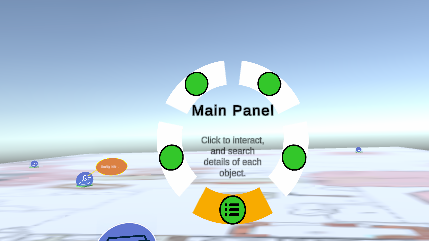
\includegraphics[width=0.8\linewidth]{Implementation/main_menu}
    \caption{Main Menu Interaction, with the option of the Main Panel selected.}
    \label{fig:main_menu}
\end{figure}

The main menu, displayed in Figure \ref{fig:main_menu}, was built with the support of the \textbf{SimplePieMenu} asset.
However, it was restructured and adapted for use with \gls{VR} controllers, since the original implementation was developed for Unity \gls{3D} without \gls{VR} handling.
The menu can be opened or closed with the trigger button of the right controller. The menu follows the user through the position of the right controller attributed in the "Follow\_Controller" script.
Additionally, to select an option, the user points at it with the ray and selects it using the right controller’s select button. To detect which menu option is being targeted, a \textbf{Raycast} operation is performed based on the current position of the right controller ray, as illustrated in Listing \ref{lst:menu_raycast}.

Currently, the menu contains only one functional option, represented by a menu icon. This option performs a single action: activating or deactivating the \textbf{Panel \gls{UI}} menu.

\begin{lstlisting}[language=C++, caption={Method used to get the position that was pointed by the controller ray.}, label={lst:menu_raycast}]
    public Vector2 GetPosition(Vector2 anchoredPosition, Transform controllerTransform)
    {
        Ray ray = new Ray(controllerTransform.position, controllerTransform.forward);
        if (Physics.Raycast(ray, out RaycastHit hit, 50f, LayerMask.GetMask("Default")))
        {
            Vector3 screenPoint = Camera.main.WorldToScreenPoint(hit.point);
            
            return new Vector2(
                screenPoint.x - Screen.width / 2f,
                screenPoint.y - Screen.height / 2f
            );
        }
        return Vector2.zero;
    }
\end{lstlisting}


\subsection*{Panel \gls{UI}}
\label{sec:panel_UI}
\begin{figure}[h!]
    \centering
    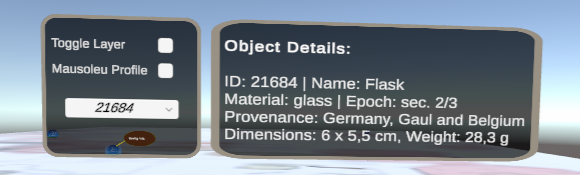
\includegraphics[width=0.8\linewidth]{Implementation/main_panel}
    \caption{Panel \gls{UI} Interaction.}
    \label{fig:main_panel}    
\end{figure}

The \gls{UI} includes a canvas where users can interact with and explore object data, as shown in the left panel of Figure \ref{fig:main_panel}. 

In this example, the object ID selected from the dropdown menu is "21684," and the textual data associated with this object is displayed in the right panel. 
This panel is initially empty and populates with the relevant object details after a selection is made. 

The \gls{UI} contains three interactive elements: the "Toggle Layer" and "Mausoleum Profile" checkboxes, and the "Dropdown Menu".

 \begin{figure}[h!]
    \centering
    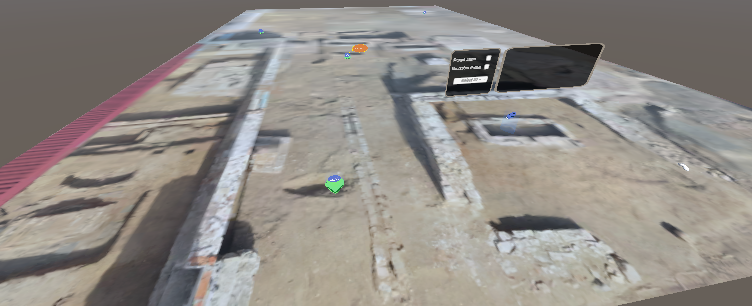
\includegraphics[width=0.8\linewidth]{Implementation/layer}
    \caption{Toggle Layer to a photo of the Site Occidental part.}
    \label{fig:toggle_layer}    
\end{figure}


 \begin{figure}[h!]
    \centering
    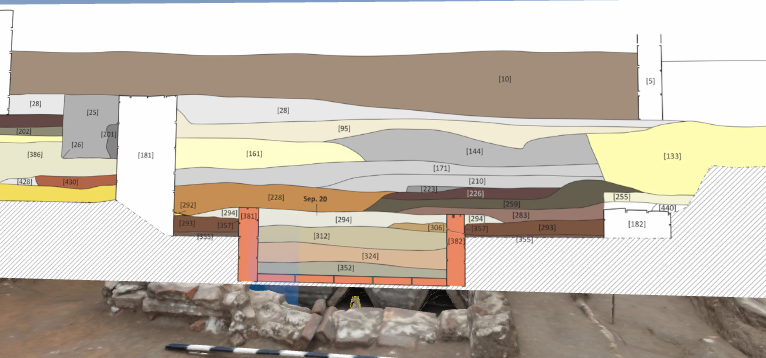
\includegraphics[width=0.8\linewidth]{Implementation/mausoleum_profile}
    \caption{Funerary Enclosure Profile constructions layer view.}
    \label{fig:mausoleum_profile}    
\end{figure}

The first element, \textbf{Toggle Layer}, is a checkbox that controls the visibility of the ground plane.
By default, the base plan is represented by a partial drawing of this archaeological site, which includes the burial enclosure under study. 
When the user activates the checkbox, the plan switches to a photograph of the actual site, offering a more realistic view and a stronger sense of presence. 
This feature is illustrated in Figure \ref{fig:toggle_layer}.
The user can at any time toggle the view in the checkbox to view the pretended plan.

The second element, the \textbf{Funerary Enclosure Profile}, demonstrated in Figure \ref{fig:mausoleum_profile}, works similarly. However, in this case, it opens a profile image of the mausoleum wall, displaying the different material types and layers of construction.

The third element, the \textbf{Dropdown Menu}, allows the user to select an object by its identification number (ID).
Once selected, the corresponding textual data and intervention images are retrieved from the database.
Besides this interaction panel, on the right side of the interface is the place where the textual data related to the selected Object ID is displayed.

The Images Gallery interaction, displayed on the left side of the map, is described below.

\subsection*{Image Gallery}
\label{sec:image_gallery}

\begin{figure}[h!]
    \centering
    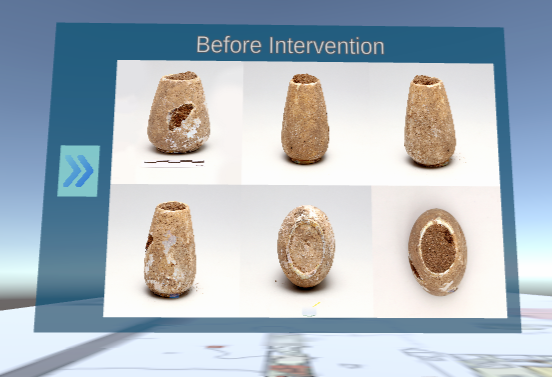
\includegraphics[width=0.7\textwidth]{Implementation/images_gallery}
    \caption{Image Gallery with object images before intervention.}
    \label{fig:image_gallery}
\end{figure}

The \gls{VE} also contains an image gallery that is activated upon object selection. 
This gallery displays images of the object before and after intervention. 
Users can switch between these states by hovering the controller ray over the gallery arrow. 
In this manner, they can view the images of a concrete object, compare the visual differences, and acquire a clearer understanding of the intervention's impact on each object.

\subsection*{Points of Interest}
\label{sec:points_interest}

\begin{figure}[h!]
    \centering
    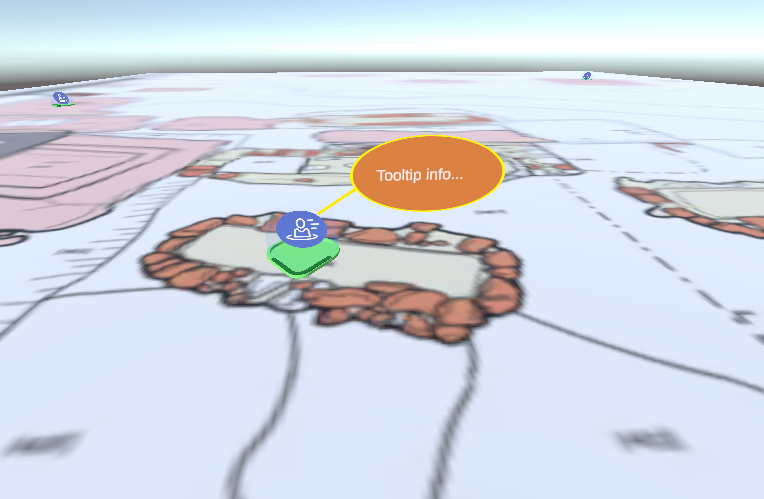
\includegraphics[width=0.7\textwidth]{Implementation/anchor_with_tool_tip}
    \caption{Exemplified point of interest with an aggregated tooltip.}
    \label{fig:points_interest}
\end{figure}

Diverse points of interest were placed in key areas across the plane.

Users can teleport directly to a point of interest by selecting a blue anchor (implemented with the default \emph{Teleportation Anchor} component) within the plan. These points are designed to draw the user’s attention to notable features or artifacts, with the most relevant point for the current study located inside the tomb within the funerary enclosure.

In the future, the idea is to expand to other points and create interactive features as the \gls{3D} funerary enclosure model. Figure \ref{fig:points_interest} illustrates one of these anchors.

\subsection*{Object Slider}
\label{sec:object_slider}

 \begin{figure}[h!]
    \centering
    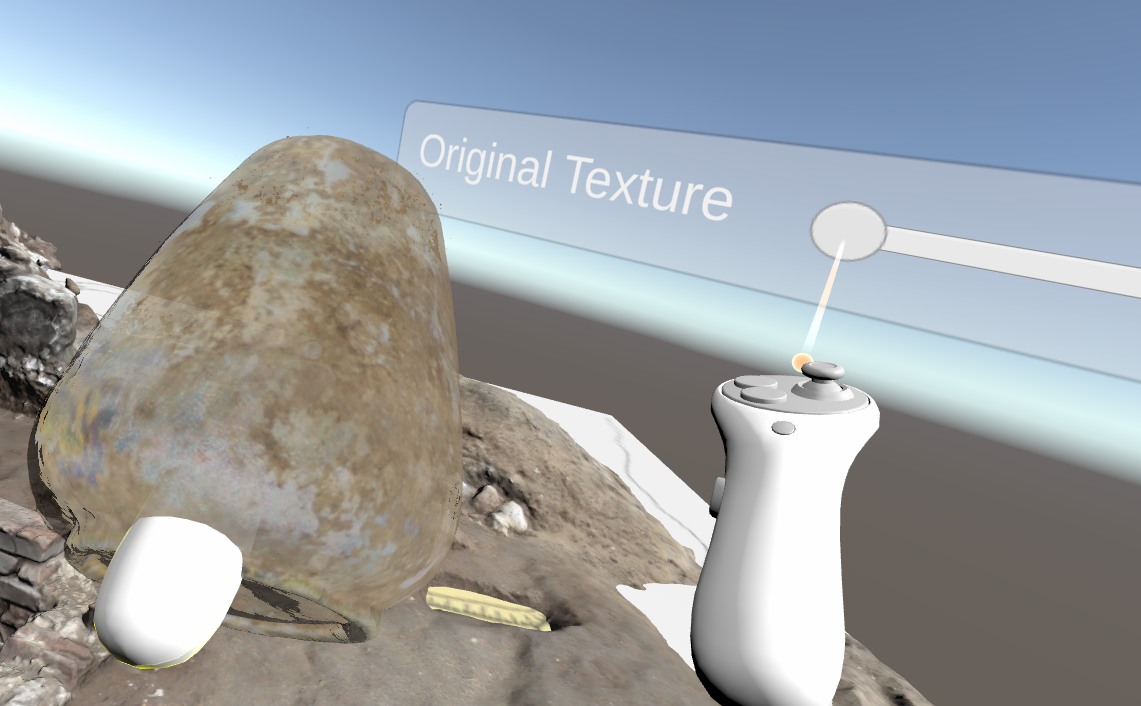
\includegraphics[width=0.8\linewidth]{Implementation/grab_object}
    \caption{Object Slider Interaction.}
    \label{fig:object_slider}
\end{figure}

The Object Slider was designed as an interactive feature within the \gls{VE}, allowing users to visualize an object's transformation over time, from its original condition to its current, restored state. 

This functionality is illustrated in Figure \ref{fig:object_slider}, where the user holds the object with the left controller while manipulating the slider, named “Original Texture,” with the right controller. 
The texture initially displayed corresponds to the post-excavation state, and as the user moves the slider to the right, it gradually transitions to the original glass texture.
The goal was to provide an immersive experience, creating the sensation of traveling back in time to observe the physical changes the object has undergone throughout the years.

Several experimental approaches were conducted to achieve this effect, focusing on shader development.
Two main approaches were explored, as described below:

The first attempt involved creating a shader that utilized a single texture input, specifically the texture of the object after restoration. A white color was used to control the alpha (transparency) values, and the transition effect was managed using a linear interpolation (lerp) function. This shader was developed using Unity’s Shader Graph, which provided a visual, node-based interface for building the transition logic.


The final solution involved a more advanced shader, written in Unity High-Level Shader Language (HLSL) for the Universal Render Pipeline (URP)\footnote{\url{https://docs.unity3d.com/Manual/urp/writing-custom-shaders-urp.html}}. 
This approach provided more control over the material's appearance compared to Unity's built-in shaders.
The shader was constructed using key URP shader libraries, including those for lighting and shading calculations\footnote{\url{https://docs.unity3d.com/Packages/com.unity.render-pipelines.universal@14.0/manual/use-built-in-shader-methods-lighting.html}}
, reflection probes\footnote{\url{https://docs.unity3d.com/Manual/urp/use-built-in-shader-methods-indirect-lighting.html}}
, shadow integration\footnote{\url{https://docs.unity3d.com/6000.1/Documentation/Manual/urp/use-built-in-shader-methods-shadows.html}}
, camera operations\footnote{\url{https://docs.unity3d.com/Manual/urp/use-built-in-shader-methods-camera.html}}
, and transformations\footnote{\url{https://docs.unity3d.com/Manual/urp/use-built-in-shader-methods-transformations.html}}.
%https://docs.unity3d.com/Manual/urp/use-built-in-shader-methods.html

This version accepted two texture inputs: the original appearance of the object (input variable \texttt{\_DecayTex}) and its current state (input variable \texttt{\_RestoredTex}).
Besides the texture inputs, the shader provides the following adjustable material properties: \emph{Blend Factor}, \emph{Smoothness}, \emph{Fresnel Power}, \emph{Specular Color}, and \emph{Reflection Intensity}, enabling precise control over how the textures blend and the visual appearance of the material. 
These properties can be modified directly through the Unity Inspector.

A \textbf{Lerp function} was used to interpolate between the two textures, considering their \texttt{Albedo}, \texttt{Alpha} and \texttt{Smoothness} attributes, as shown in Listing \ref{lst:shader_blend}. %based on the user's interaction with the virtual slider. 

To enhance realism, additional lighting and reflection techniques were integrated into the shader, including 
the \textbf{Fresnel Effect}\footnote{\url{https://docs.unity3d.com/Packages/com.unity.shadergraph@6.9/manual/Fresnel-Effect-Node.html}} to model light behaviour based on the angle between the surface normal (\texttt{normalWS}) and the view direction (\texttt{viewDirWS}), 
and adjustments to \textbf{specular}, \textbf{diffuse}, and \textbf{environment lighting} properties. 
These calculations were performed independently for each component, as illustrated in Listing~\ref{lst:lighting_glass}, before being aggregated into the final \texttt{finalColor}. 
This shader enabled a more faithful representation of the object's original appearance.

\begin{lstlisting}[language=HLSL, caption={Partial Fragment shader for blending original and restored textures.}, label={lst:shader_blend}]
        half4 frag(Varyings IN) : SV_Target
        {
            half4 decayAlbedo = SAMPLE_TEXTURE2D(_DecayTex, sampler_DecayTex, IN.uv);
            half4 restoredAlbedo = SAMPLE_TEXTURE2D(_RestoredTex, sampler_RestoredTex, IN.uv);

            float3 normalWS = normalize(IN.worldNormal);
            float3 viewDirWS = normalize(IN.viewDirWS);

            float fresnel = CalculateFresnel(normalWS, viewDirWS, _FresnelPower);

            half3 finalAlbedo = lerp(decayAlbedo.rgb, restoredAlbedo.rgb, _BlendFactor);
            half finalAlpha = lerp(decayAlbedo.a, restoredAlbedo.a, _BlendFactor);
            half finalSmoothness = lerp(_GlassSmoothness, _RestoredSmoothness, _BlendFactor);
            ... Populate Data...
            
            half3 glasslitColor = CalculateGlassLighting(surfaceData, inputData, fresnel);            
            half enhancedAlpha = lerp(finalAlpha, finalAlpha * 0.5, fresnel * 0.5);
            
            return half4(glasslitColor, enhancedAlpha);
        }
\end{lstlisting}


\begin{lstlisting}[language=C++, caption={Lighting Glass Texture Partial Calculation.}, label={lst:lighting_glass}]
  float3 CalculateGlassLighting(SurfaceData surfaceData, InputData inputData, float fresnel)
  {
      Light mainLight = GetMainLight(inputData.shadowCoord, inputData.positionWS, inputData.shadowMask);
      ...

      float3 specular = specularTerm * mainLight.color * _SpecularColor.rgb * surfaceData.smoothness;
      ...

      float3 diffuse = lerp((surfaceData.albedo * mainLight.color * NdotL * 0.1),surfaceData.albedo, _BlendFactor);
      ...     

      float3 environmentReflection = GlossyEnvironmentReflection(reflectionVector, 
          inputData.positionWS, surfaceData.smoothness, 1.0) * _ReflectionIntensity;

      float3 finalColor = diffuse + (specular + environmentReflection * fresnel);
      
      return finalColor;
  }
\end{lstlisting}

\subsection*{Object Outline}
\label{sec:object_outline}

 \begin{figure}[h!]
    \centering
    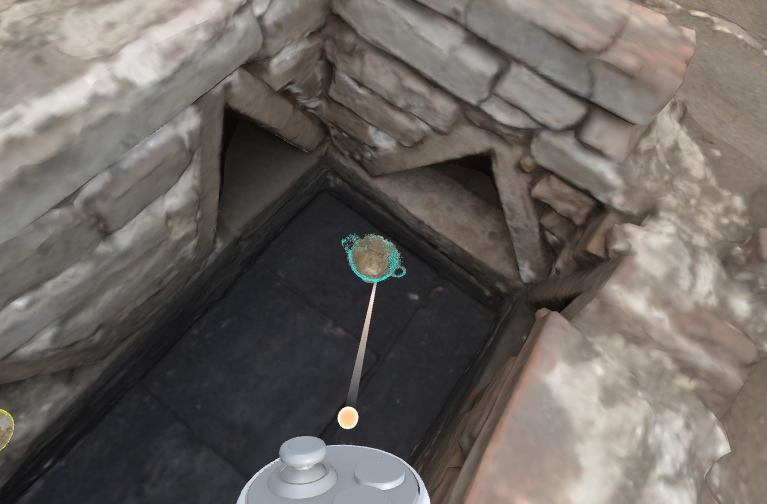
\includegraphics[width=0.8\linewidth]{Implementation/outline_object}
    \caption{Outline effect applied when an object is hited with the controller ray.}
    \label{fig:outline_object}    
\end{figure}


This functionality was implemented to improve the visibility of objects within the tomb and to distinguish them from the surrounding funerary ground.  
It essentially consists of an outline shader and a complementary script that manages its parameters. 
The shader highlights objects when targeted with the controller ray, as illustrated in Figure~\ref{fig:outline_object}

The shader includes the following input parameters: \emph{Outline Color}, \emph{Outline Width}, \emph{Outline Power}, and \emph{Outline Softness}.  
Similar to the shader described for the Object Slider functionality in Section~\ref{sec:object_slider}, this shader also relies on the Fresnel effect to control outline intensity and appearance.  

The rendering of each object includes two materials: a primary material representing its texture and a secondary material responsible for the outline effect.
When the user points at the object, the parameter \texttt{OutlineColor} is switched from yellow to blue. But if the object is not being grabbed (\texttt{if(!select)}), the outline disappears. 
This behavior is handled through hover events, as shown in Listing~\ref{lst:outline_color}. 
By accessing the second material of the object via \texttt{meshRenderer.materials[1]}, the shader updates the outline color.  

The fragment shader logic for the glowing outline is presented in Listing~\ref{lst:outline_effect}. 
It computes the Fresnel term with the Outline Power attribute, and applies a \texttt{smoothstep()} to achieve a soft personalized outline.  
This mechanism ensures that the objects are easily identifiable. 


\begin{lstlisting}[language=C++, caption={Partial class with Outline Color changed when the object is Hovered.}, label={lst:outline_color}]
    public class GlowingObject : MonoBehaviour
{
    private MeshRenderer meshRenderer;
    private bool select = false;
    Color Yellow = new Color(65, 65, 0, 1);
    Color Blue = new Color(0, 59, 49, 1);
    ...
    public void OnHoverEnter()
    {
        meshRenderer.materials[1].SetColor("_OutlineColor", Blue);
    }

    public void OnHoverExit()
    {
        if(!select)
            meshRenderer.materials[1].SetColor("_OutlineColor", Yellow);
    }
    ...
}
\end{lstlisting}


\begin{lstlisting}[language=HLSL, caption={Partial Fragment shader for creating an outline effect to the object.}, label={lst:outline_effect}]
        float4 frag(v2f i) : SV_Target
        {
            float3 N = normalize(i.normalWS);
            float3 V = normalize(i.viewDirWS);

            float fresnel = pow(1.0 - saturate(dot(N, V)), _OutlinePower);

            float edge1 = 1.0 - _OutlineWidth;
            float edge2 = edge1 + _OutlineSoftness;
            float outlineFactor = smoothstep(edge1, edge2, fresnel);

            return _OutlineColor * outlineFactor;
        }
\end{lstlisting}

\subsection*{Grab and Release Object}
\label{sec:object_interaction}

The artefacts can be grabbed with the lateral button of the controllers.
When the object is grabbed or released, the corresponding event in Listing~\ref{lst:grab_release} is triggered.  

The proximity of the controller's ray to the object determines how close the object appears to the user's view. 
Releasing the object is achieved simply by releasing the button.  
Small objects are automatically zoomed when hovered over or grabbed (operation \texttt{transform.localScale = zoomScale}), improving clarity and visibility during interaction.

Additionally, two other behaviors are implemented. 
The colliders that might interfere during grabbing are reactivated upon release, except when the user is inside the tomb, in which case a coroutine (\texttt{StartCoroutine}) is executed.
During \texttt{OnGrab}, and as illustrated in Figure \ref{fig:object_slider}, the object slider is repositioned depending on whether the object is grabbed with the left or right controller, controlled by the \texttt{CompareTag} method.

\begin{lstlisting}[language=C++, caption={Partial Fragment of objects onGrab and onRelease events.}, label={lst:grab_release}]
     
    private void OnGrab(SelectEnterEventArgs args)
    {
        transform.localScale = zoomScale;
        args.interactableObject.colliders.ForEach(collider => { collider.enabled = false; });
        ...
        var interactor = args.interactorObject.transform;
        if (interactor.CompareTag("left")) 
        {
            follow.targetOffset = new Vector3(sliderRightxPos, follow.targetOffset.y, follow.targetOffset.z);
        }
        else if (interactor.CompareTag("right")) 
        {
            follow.targetOffset = new Vector3(sliderLeftxPos, follow.targetOffset.y, follow.targetOffset.z);
        }
    }

    private void OnRelease(SelectExitEventArgs args)
    {
        transform.localScale = originalScale;
        args.interactableObject.colliders.ForEach(collider => { collider.enabled = true; });
        ...
        if (r.isInsideTomb)
        {
            StartCoroutine(DisableColliderRoutine(5f));
        }
        ...
    }
\end{lstlisting}


\subsection*{Funerary Enclosure Interaction}
\label{sec:funerary_interaction}

 \begin{figure}[h!]
    \centering
    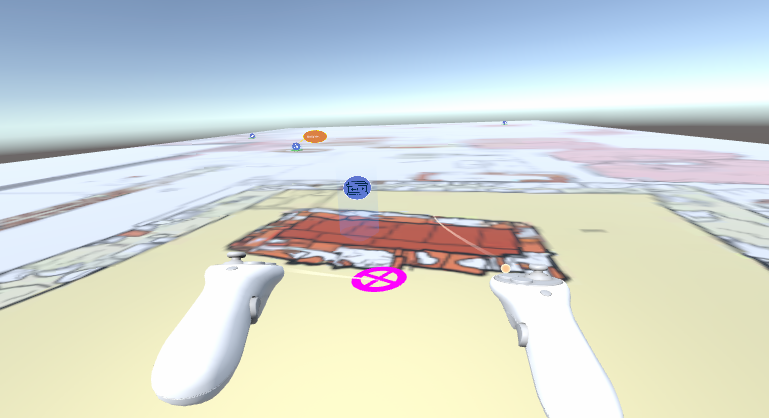
\includegraphics[width=0.8\linewidth]{Implementation/default_plan_with_reticle}
    \caption{Funerary Enclosure Activation Reticle in the default ground plan.}
    \label{fig:funerary_interaction}    
\end{figure}

The system provides the possibility to activate or deactivate the \gls{3D} model of the funerary enclosure.
This functionality is triggered using the trigger button of the left command. When the user points to the funerary enclosure area in the map, a purple reticle appears, indicating that the enclosure can be activated, as illustrated in Figure \ref{fig:funerary_interaction}. This interaction can be performed at any point during the experience.

To ensure realism, the funerary enclosure is implemented with a default \emph{Mesh Collider} combined with an aggregated \emph{Rigidbody}. This configuration prevents the user from crossing the enclosure walls and accurately reproduces the surface levels of the original structure, thereby enhancing the immersive experience.

An exception occurs when the user is inside the tomb. In this case, the funerary enclosure collider is temporarily disabled, allowing the user to descend naturally to the ground without obstruction. Once the user exits the tomb, the collider is restored to maintain consistent collision detection.

\subsection*{User Navigation}
\label{sec:user_navigation}

The user can navigate in the environment with the controllers. 
These allow two modes of movement: continuous walking, which simulates real-world locomotion, and teleportation, providing a faster way to reposition within the scene.

There are two types of teleportation available in the environment. The first allows the user to teleport freely to any position on the environment’s ground plane (default \emph{Teleportation Area} component). The second restricts teleportation to specific points of interest, marked with blue icons (anchors).

In addition to locomotion, users can switch their perspective inside the environment, using the controllers, moving laterally with the right joystick.
Both continuous movement and snap turning can also be performed physically, without controllers, within the limits of the real-world space.

The overall movement system is managed by the \emph{Character Controller} component, which also ensures accurate collision detection. In particular, the collider associated with the user interacts with the collider of the funerary enclosure, preventing the user from passing through walls and thereby preserving realism in the experience.

Further refinements and a dynamic management of movement behavior were introduced in the script "CustomMovement", where two key methods were implemented within Unity’s default \texttt{Update()} function.
The first method continuously updates the center of the character controller to reflect the user’s current position during locomotion. 
The second manages custom movement behaviors by dynamically controlling gravity. Depending on the context, gravity may either be applied or disabled. When active, it influences the user’s velocity over time, and its intensity can be adjusted dynamically.

\subsection*{Tomb Navigation Logic}
\label{sec:tomb_logic}

 \begin{figure}[h!]
    \centering
    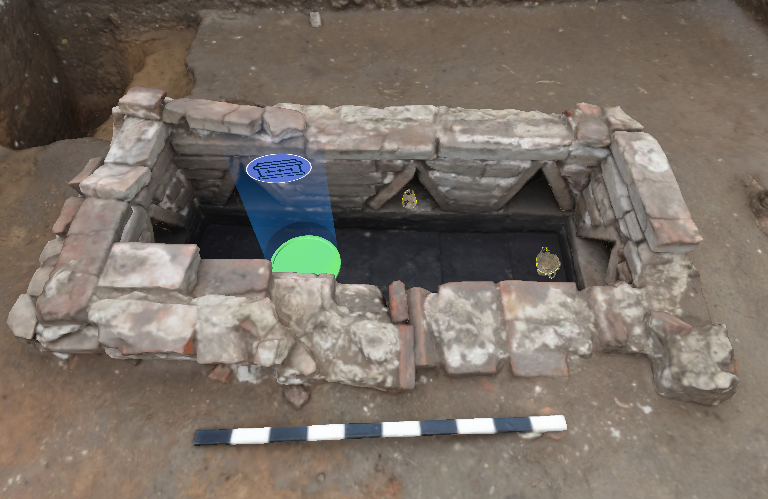
\includegraphics[width=0.8\linewidth]{Implementation/tomb_outside}
    \caption{Tomb Exterior View with blue anchor inside.}
    \label{fig:tomb_outside}    
\end{figure}

 \begin{figure}[h!]
    \centering
    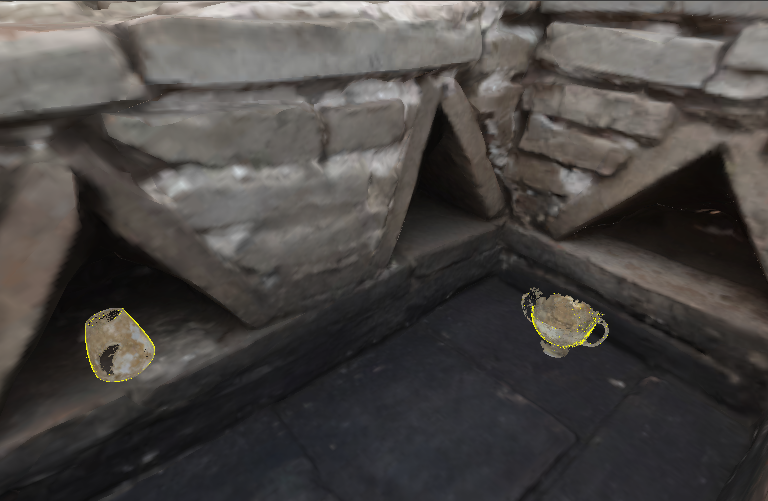
\includegraphics[width=0.8\linewidth]{Implementation/tomb_inside}
    \caption{Tomb Interior View with Objects positioned.}
    \label{fig:tomb_inside}    
\end{figure}

To access the tomb, the user may either walk in continuous movement toward its interior or use teleportation by clicking on the blue anchor located in that area.
Upon entering, the user will have a view similar to the one shown in Figure \ref{fig:tomb_inside}.
The tomb contains triangular areas, that was the place where the majority of the objects were discovered. 
It's important to note that the artifacts are presented in the exact positions in which they were found during the excavations.
During the dissertation process, different techniques were implemented and tested to address navigation and visualization challenges inside the tomb.

\begin{enumerate}
\item{\textbf{Plan Removal}

The first approach used a collider placed inside the tomb. When the user collided with it, the ground plane was removed, revealing the full interior of the tomb.

This, in the end, caused conflicts because the interior collider overlapped with the collider responsible for activating the funerary enclosure.

To handle this issue, the limits of the tomb were defined manually. With this method, the plane disappears when the user enters that space and reappears once the user exits it.
In Figure \ref{fig:tomb_outside}, the outside view of the tomb is depicted. As illustrated, the plane is disabled, providing full visibility of the tomb’s interior.
}
\item{
\textbf{Vertical Descend}

Another challenge was ensuring that users could navigate naturally within the tomb while maintaining clear visibility of objects and architectural details inside. Standard gravity alone was insufficient, as it did not allow reliable interaction with objects located in triangular areas.
To address this, the "TombNavigation" script was developed, introducing controlled vertical displacement along the y-axis.

Initially, a Raycasting approach was tested, directing rays toward the front and the floor of the tomb. When a collision was detected, the user’s position was adjusted and lowered by a few centimeters. Although functional, this method is unreliable, as it heavily depends on the user’s viewing direction, extracted from the camera position.

The final implementation instead defined the tomb interior using axis-based boundaries. When the user entered this delimited area, they were automatically displaced downward. Upon exiting, the user’s position was restored to its correct height, ensuring they did not remain unnaturally below the expected level. This approach allows the user to enter and exit the tomb by simply walking.

During development, two alternative exit mechanisms, a block and a ladder, were added. However, these were later deactivated, as they were unnecessary with the finalized gravity-based solution and occupied additional space in the relatively small tomb environment. Nevertheless, both alternatives remain available for reactivation if required in the future.
}
\end{enumerate}


%Essential Stages/Steps
\subsection{Key Techniques}
\subsubsection{Light Technique}
There is a main directional light that illuminates the entire environment along, simulating reality. However, it was understood that depending on the angle, the user might see the tomb and objects black due to shadows. To address this, a secondary point light was added that follows the user, so the user can view the tomb with clarity and have a good visibility while navigating in the environment.

\subsubsection{Funerary Enclosure Model Reduction}
The resolution of the burial site model was significantly reduced in \emph{Agisoft Metashape} software through "Decimate Model" property.
This adjustment was necessary due to warnings of potential collision issues arising in the model's size of over 2 million triangles. 
Therefore, the number of faces was reduced from 1.9 million to approximately 100 thousand, preserving the essential level of detail while improving efficiency.

\subsubsection{Generating the Glass Texture}
The process of generating the glass texture consisted of two phases.  

First, the material was modeled in Blender using a node-based shader structure. The desired glass effect was achieved by combining the \texttt{Glossy BSDF} and \texttt{Refraction BSDF} nodes. It also received a \texttt{Fresnel} node as input\footnote{\url{https://docs.blender.org/manual/en/latest/render/shader_nodes/index.html}}. This structure is represented in Figure~\ref{fig:glass_texture}.  

After having the node structure, a UV unwrapping\footnote {\url{https://docs.blender.org/manual/en/latest/modeling/meshes/uv/unwrapping/}} was made to prepare the \gls{3D} object surface for texture mapping, process illustrated in Figure \ref{fig:uv_process}.
 Finally, a baking process\footnote{\url{https://docs.blender.org/manual/en/latest/render/cycles/baking.html}} was performed using the Cycles render engine.
With these materials, a "Combined" texture was baked and imported to Unity as a .png file.

 \begin{figure}[h!]
    \centering
    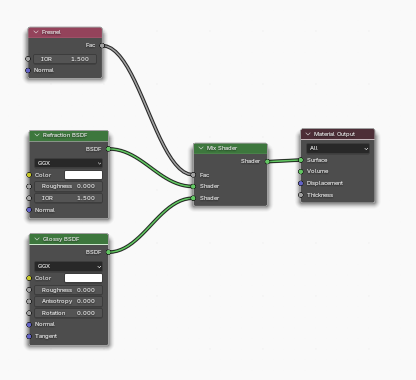
\includegraphics[width=0.8\linewidth]{Implementation/Glass_texture}
    \caption{Glass Material Nodes Blender.}
    \label{fig:glass_texture}    
\end{figure}


\begin{figure}[h!]
    \centering
    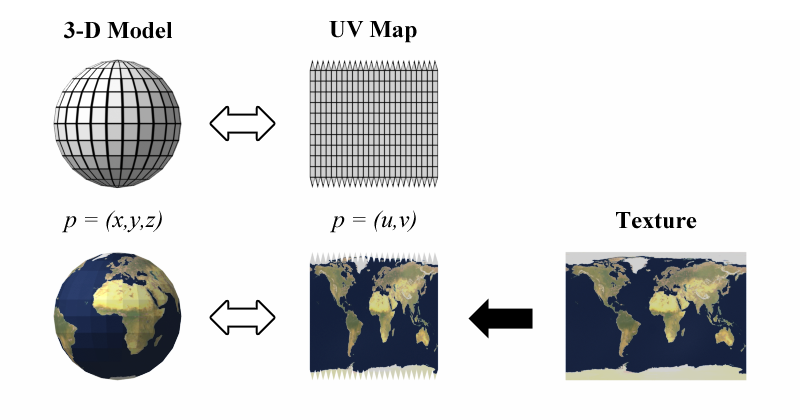
\includegraphics[width=0.8\textwidth]{Implementation/UVMapping}
    \caption{UV unwrapping process with corresponding mapped texture.}
    \label{fig:uv_process}
\end{figure}


In Unity, one \textbf{Reflection Probe} for each object was added to simulate the environment's reflection on the glass surface.
Additionally, the four attributes \emph{\_GlassSmoothness}, \emph{\_FresnelPower}, \emph{\_SpecularColor}, and \emph{\_ReflectionIntensity}, used in the slider shader in Section \ref{sec:object_slider}, can be adjusted to control the pretended reflections in the glass.
The final glass texture exemplifying one object is illustrated in Figure \ref{fig:glass1}.

\begin{figure}[h!]
    \centering
    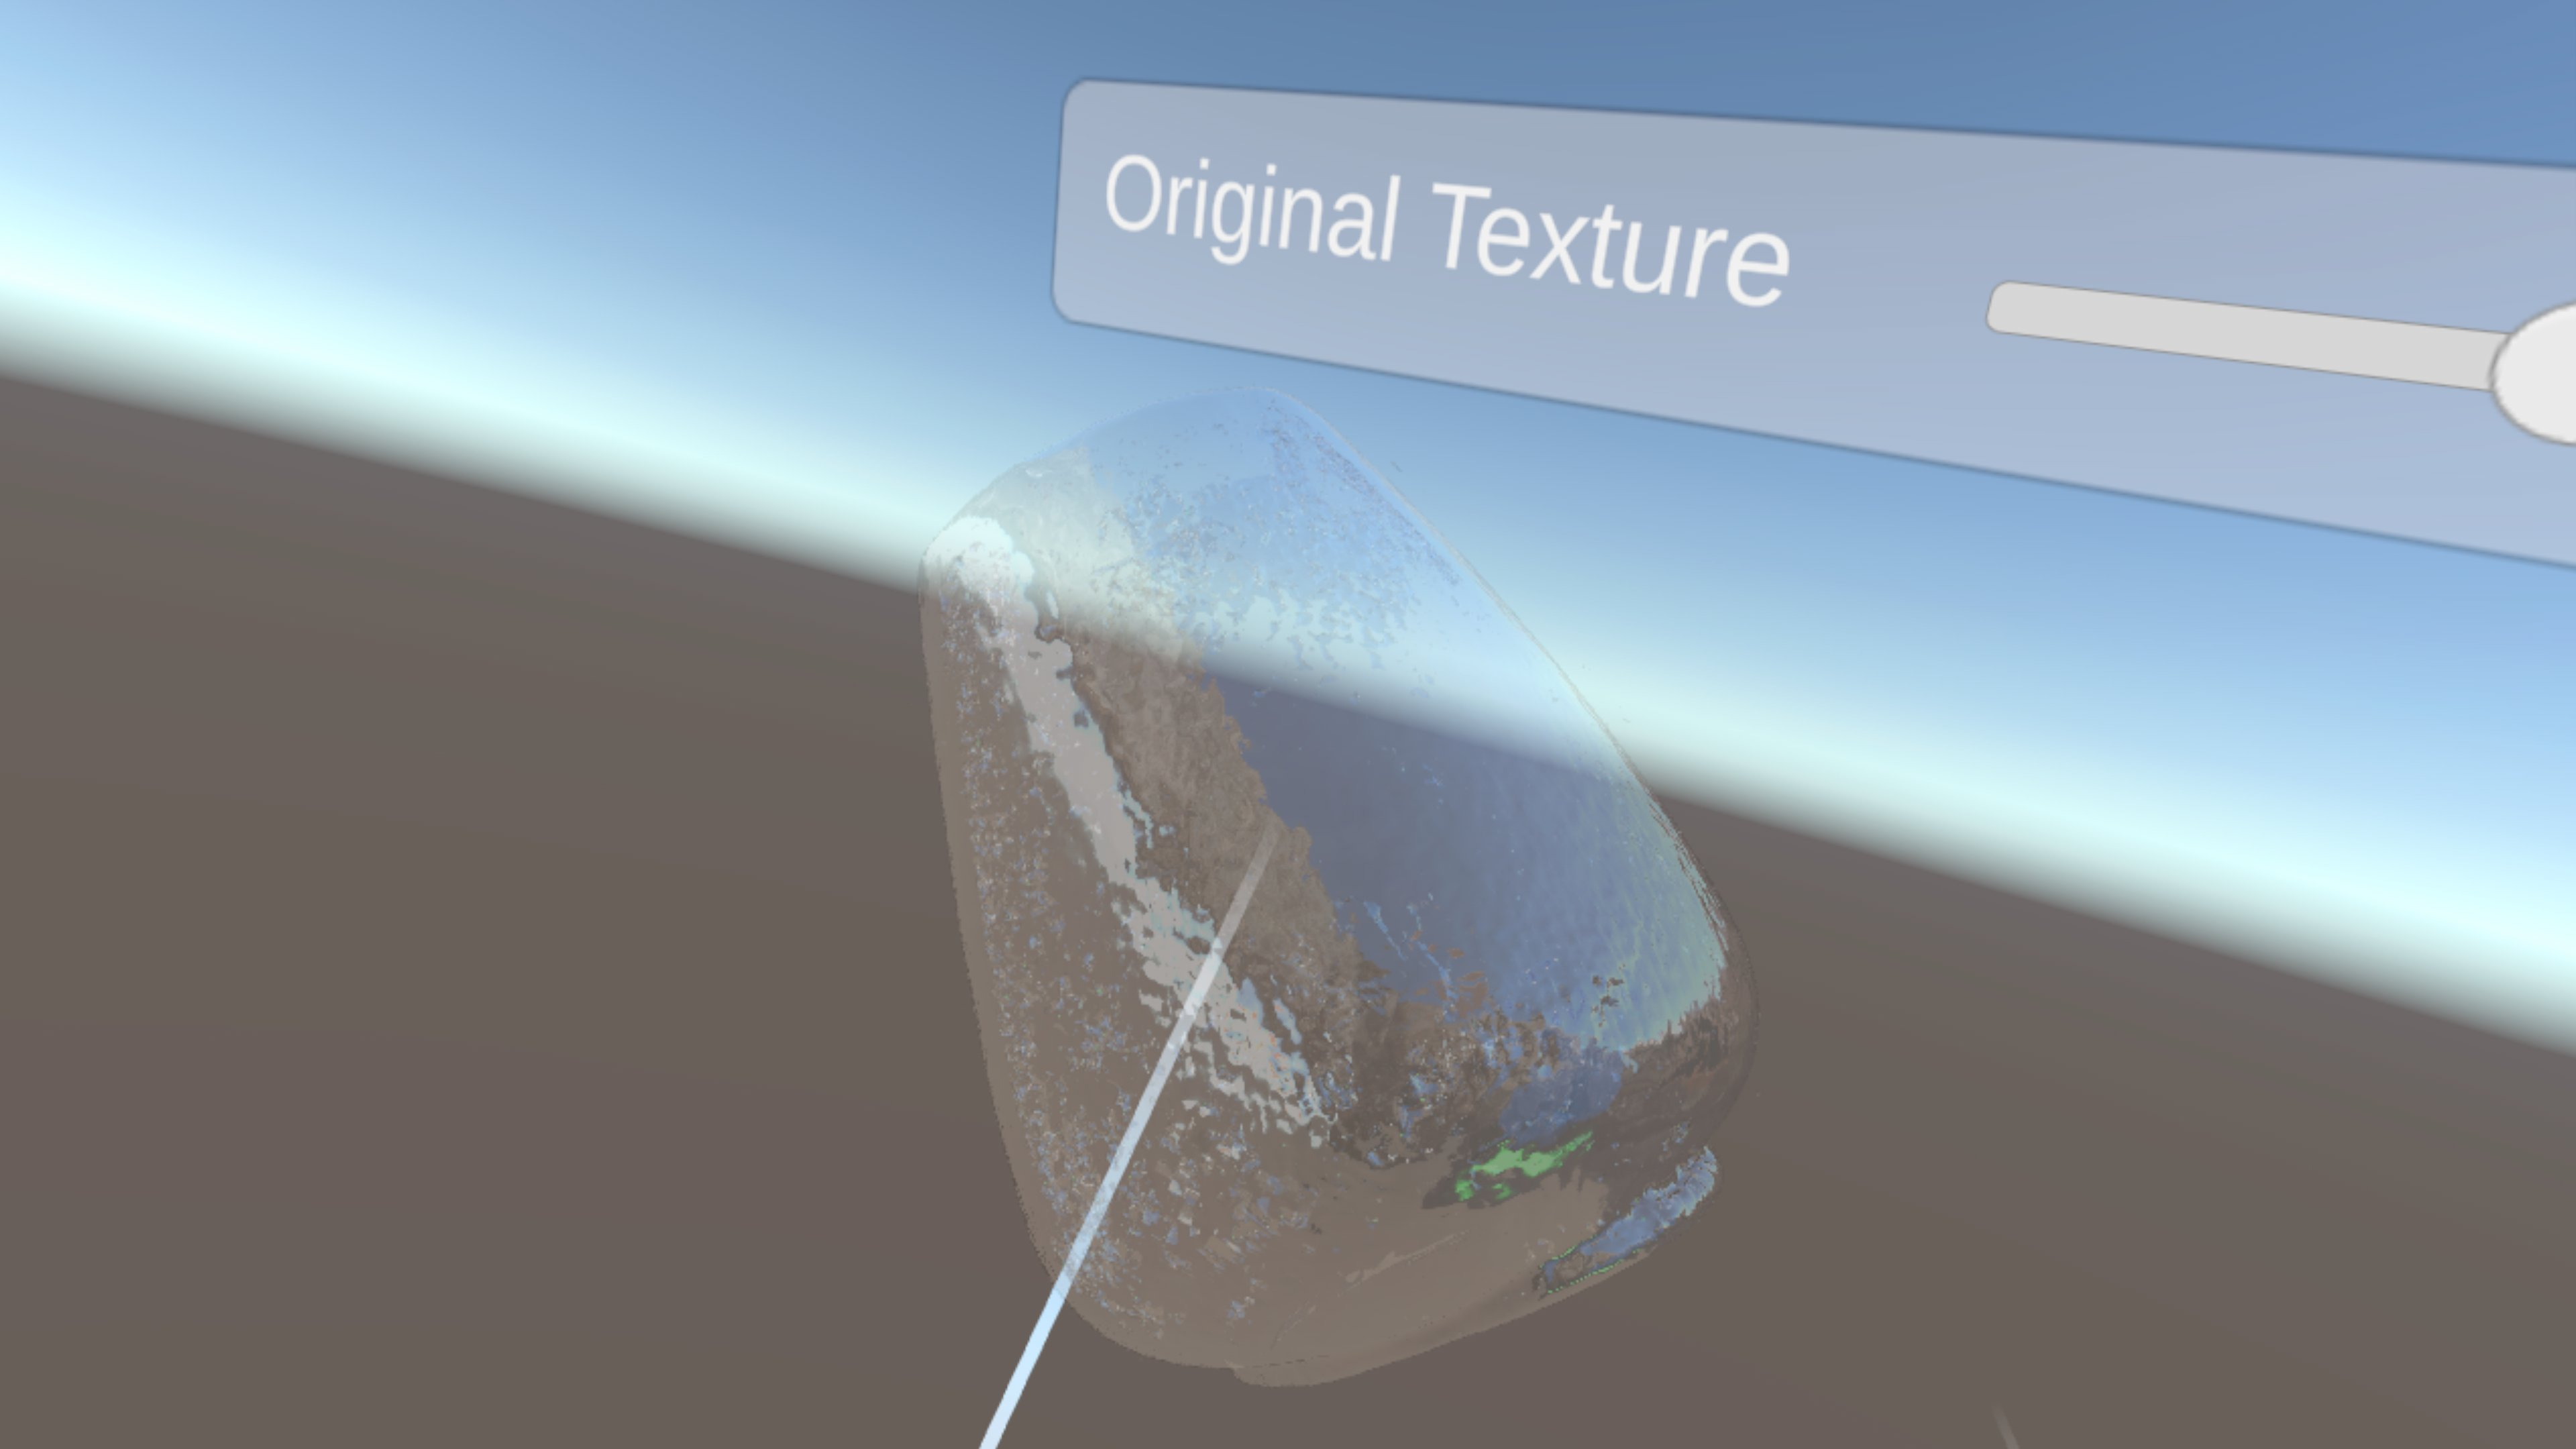
\includegraphics[width=0.8\textwidth]{Implementation/glass_1}
    \caption{Glass Texture of Object with ID 21684.}
    \label{fig:glass1}
\end{figure}


% \begin{figure}[h!]
%     \centering
%     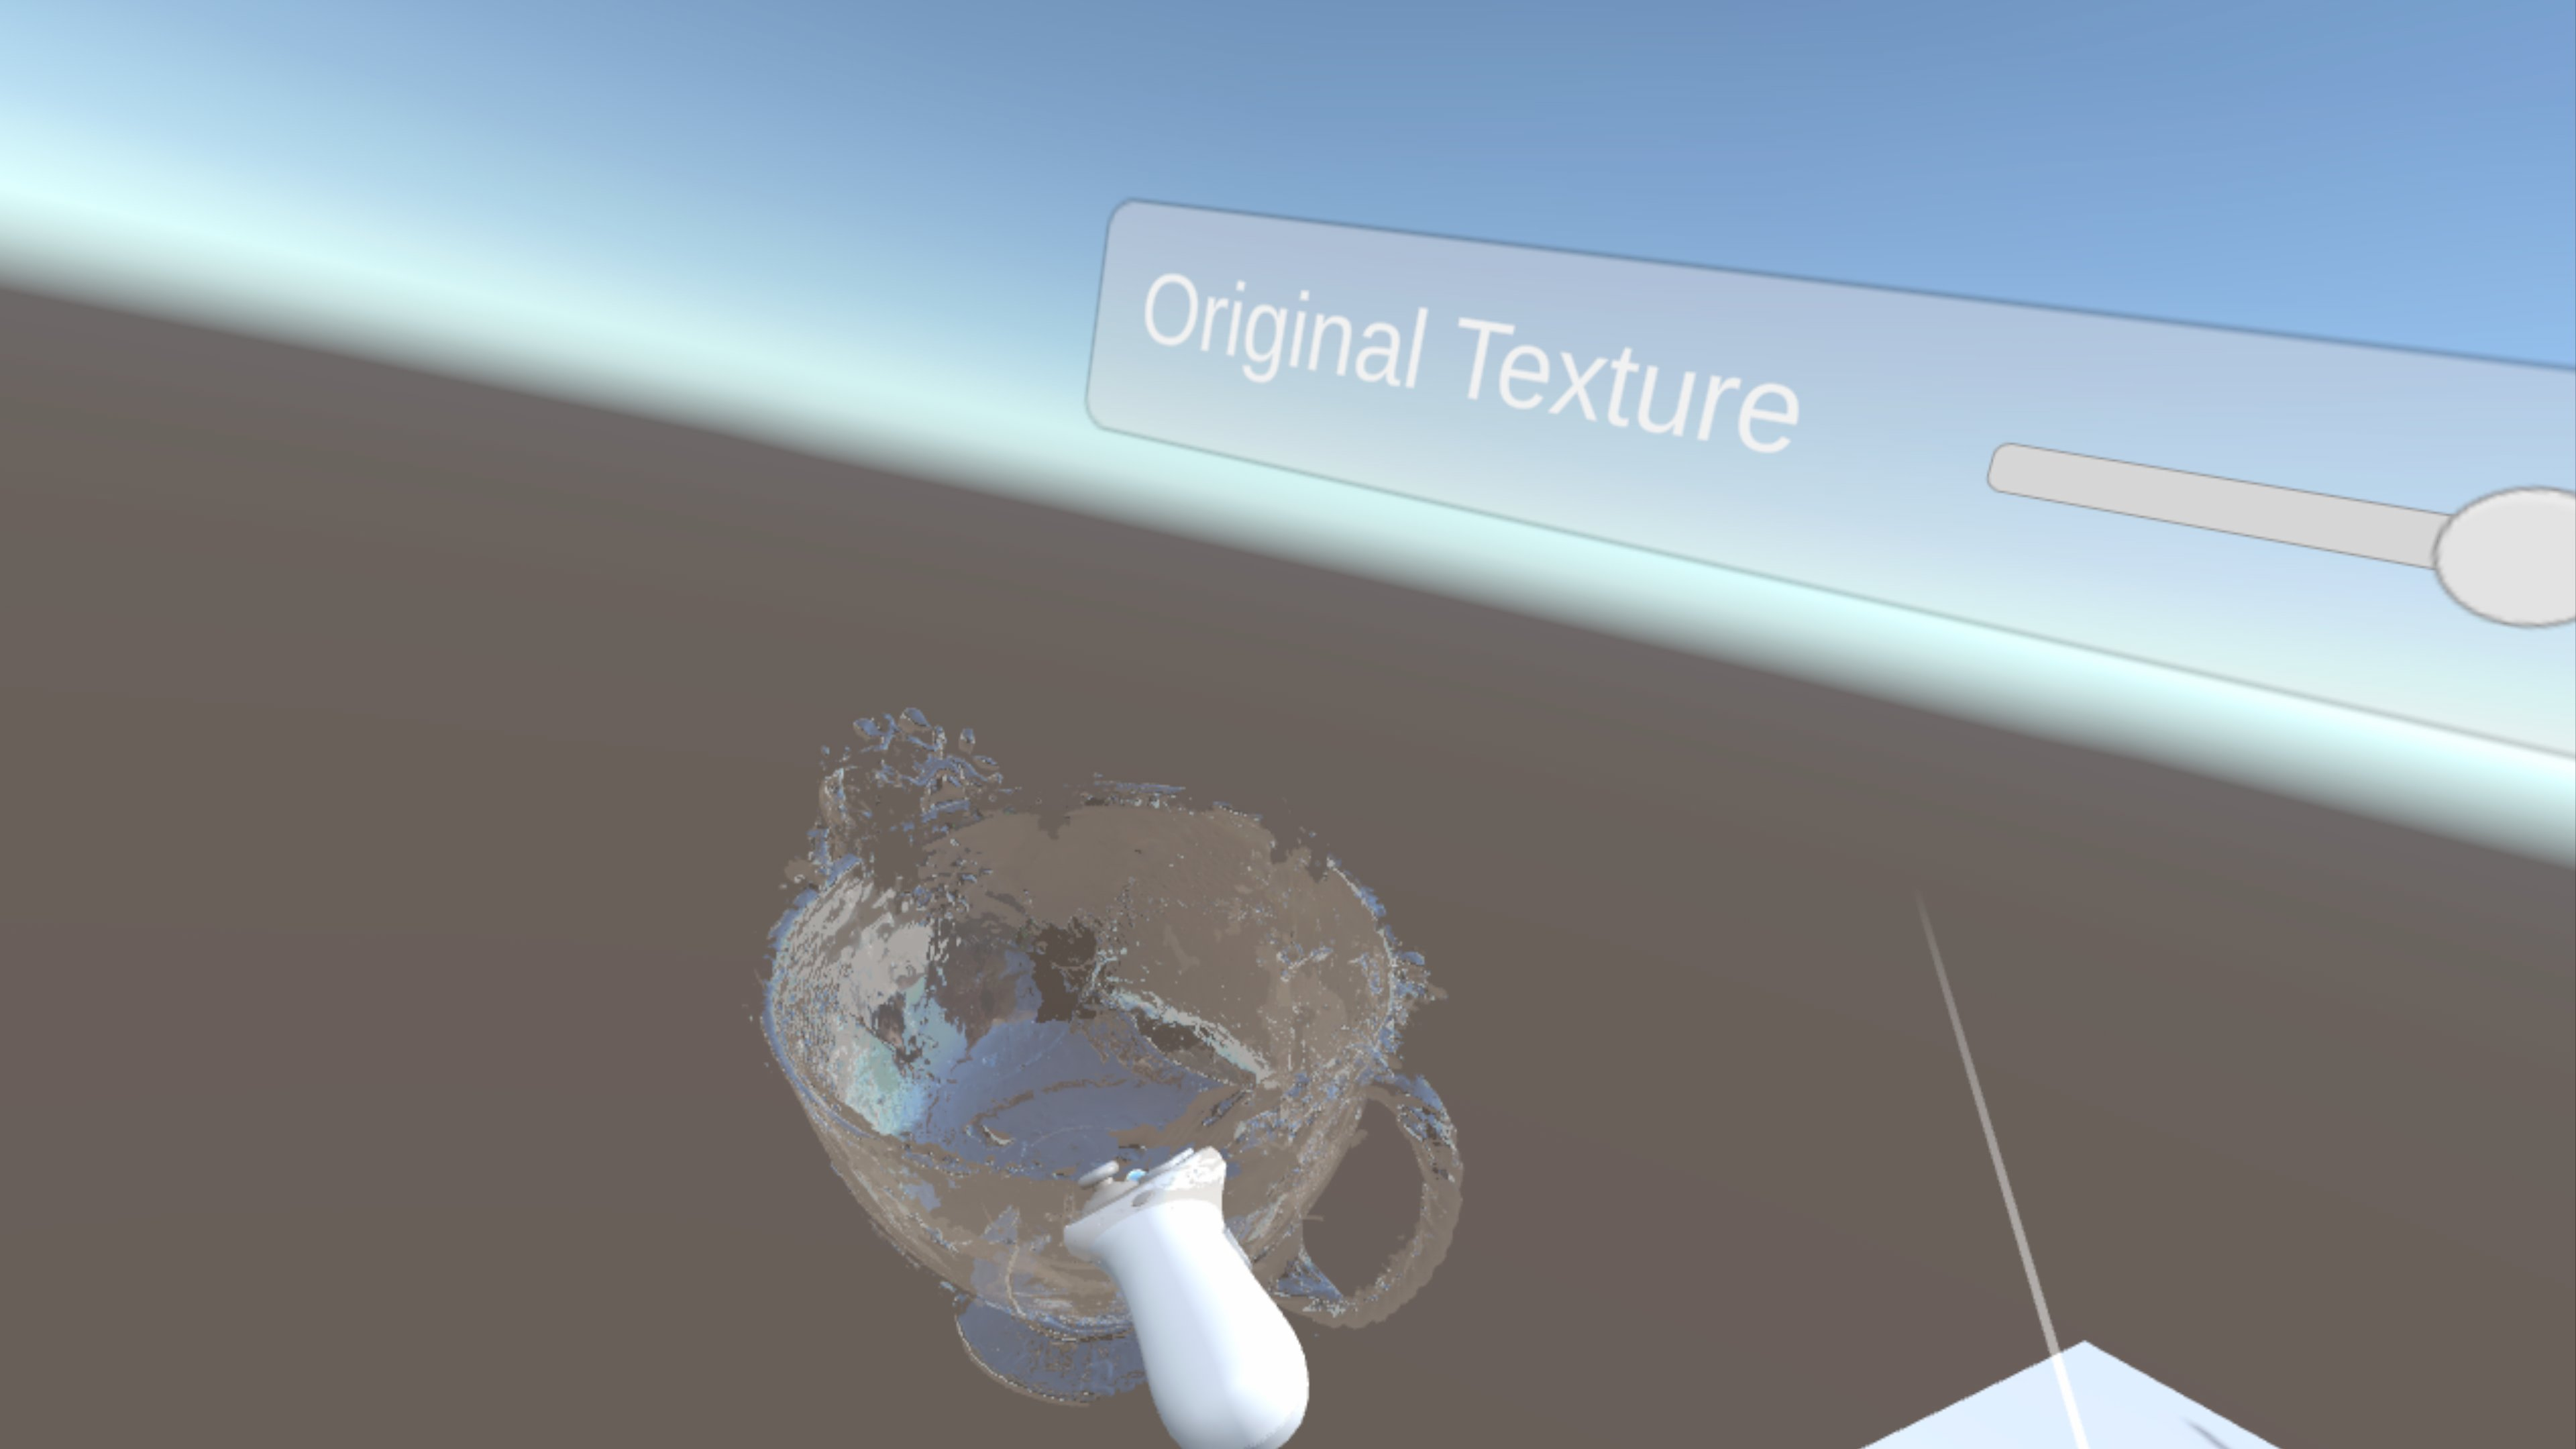
\includegraphics[width=0.8\textwidth]{Implementation/glass_2}
%     \caption{Glass Texture of Object with ID 21676.}
%     \label{fig:glass2}
% \end{figure}

\subsubsection{Generating the Funerary \gls{3D} Model}
\label{sec:build_model}

The funerary enclosure model was generated with the support of the photogrammetric survey and subsequently imported into the \textit{Sketchfab} viewer for intuitive interaction.
Within the grave, three open triangular areas were identified, containing the precious artefacts of the deceased, as shown in Figure~\ref{fig:model3} below.

This phase used the \textit{Agisoft Metashape} to stitch together photographs and capture the geometry, texture, and visual characteristics of the physical funerary structure.

The workflow began with the Align Photos operation, which produced 91,053 tie points. Then, a dense point cloud was generated to refine the level of detail, followed by the creation of a \gls{3D} mesh. The resulting model comprised 1,910,026 faces, for which a texture was mapped.
Finally, the model was exported in \texttt{.obj} format, and grouped with \texttt{.png} texture files, and imported into the Unity \gls{VR} environment.

\begin{figure}[h!]
    \centering
    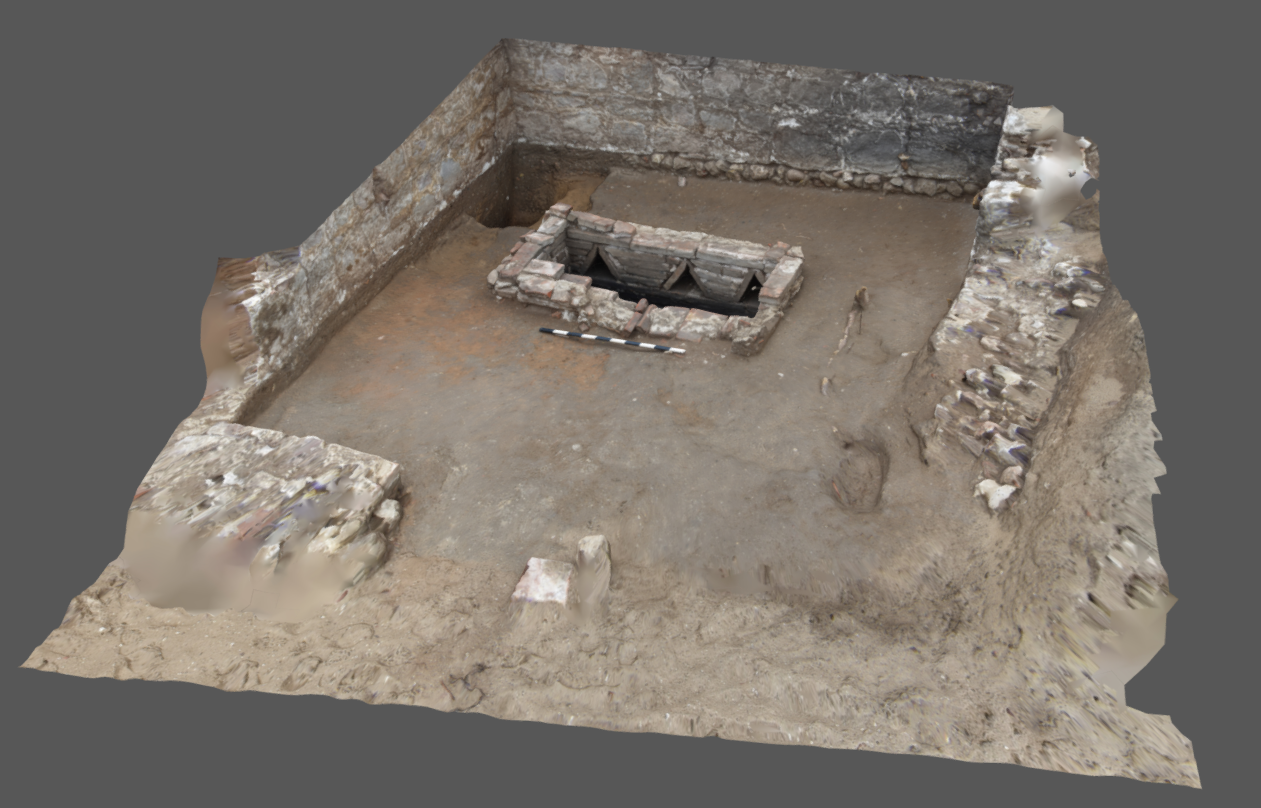
\includegraphics[width=0.7\textwidth]{model3}
    \caption{\gls{3D} Model in Sketchfab.}
    \label{fig:model3}
\end{figure}
%\section{Site Map and Data Upload}
%The map was developed having the basis of the project developed by me and Afonso, consisted on a map containing demographic ....buscar no relatório do projeto
%This way we could dedicate our time to improving and complementing the implementation as well focusing in the VE.

%\subsection{Map Functionalities}
%\subsection{Files Upload}

\subsection{Testing and Debugging}

One of the most relevant features during the development phase on controller support was the \textbf{XR Device Simulator} included in XR Interaction Toolkit. 
This utility allowed for testing \gls{VR} interactions without the need for a physical \gls{HMD}. 
It simulated input from \gls{VR} controllers using a standard mouse and keyboard. 
Despite its usefulness along this dissertation, it's important to note that certain interactions did not behave identically compared to testing with the actual headset.

During the dissertation, the functionalities within the environment were tested in real-time using the \emph{MetaLink} app. However, when connected via Wi-Fi, the environment did not load correctly. This issue was resolved by employing a wired connection.

Additionally, debugging was performed with the Visual Studio debugger and Android Debug Bridge (adb). This second tool enabled a deeper debugging and the identification of issues in the interaction with the headset by accessing detailed system logs through the \texttt{adb logcat} command. The logs proved useful for tracing errors and understanding their source during testing.

\section{Database Management}
\label{sec:database}

\subsection{Data Structure}

The database consists of 11 tables that ensure the significant data of excavation and objects are stored. %All artefacts data, excavation details, and objects intervention data were stored within this repository.
These tables cover data on the necropolis, funerary enclosure, tombs, objects, excavations, and interventions.
The detailed structure, including relationships and attributes, is illustrated in Figure \ref{fig:database}.

\begin{figure}[h!]
    \centering
    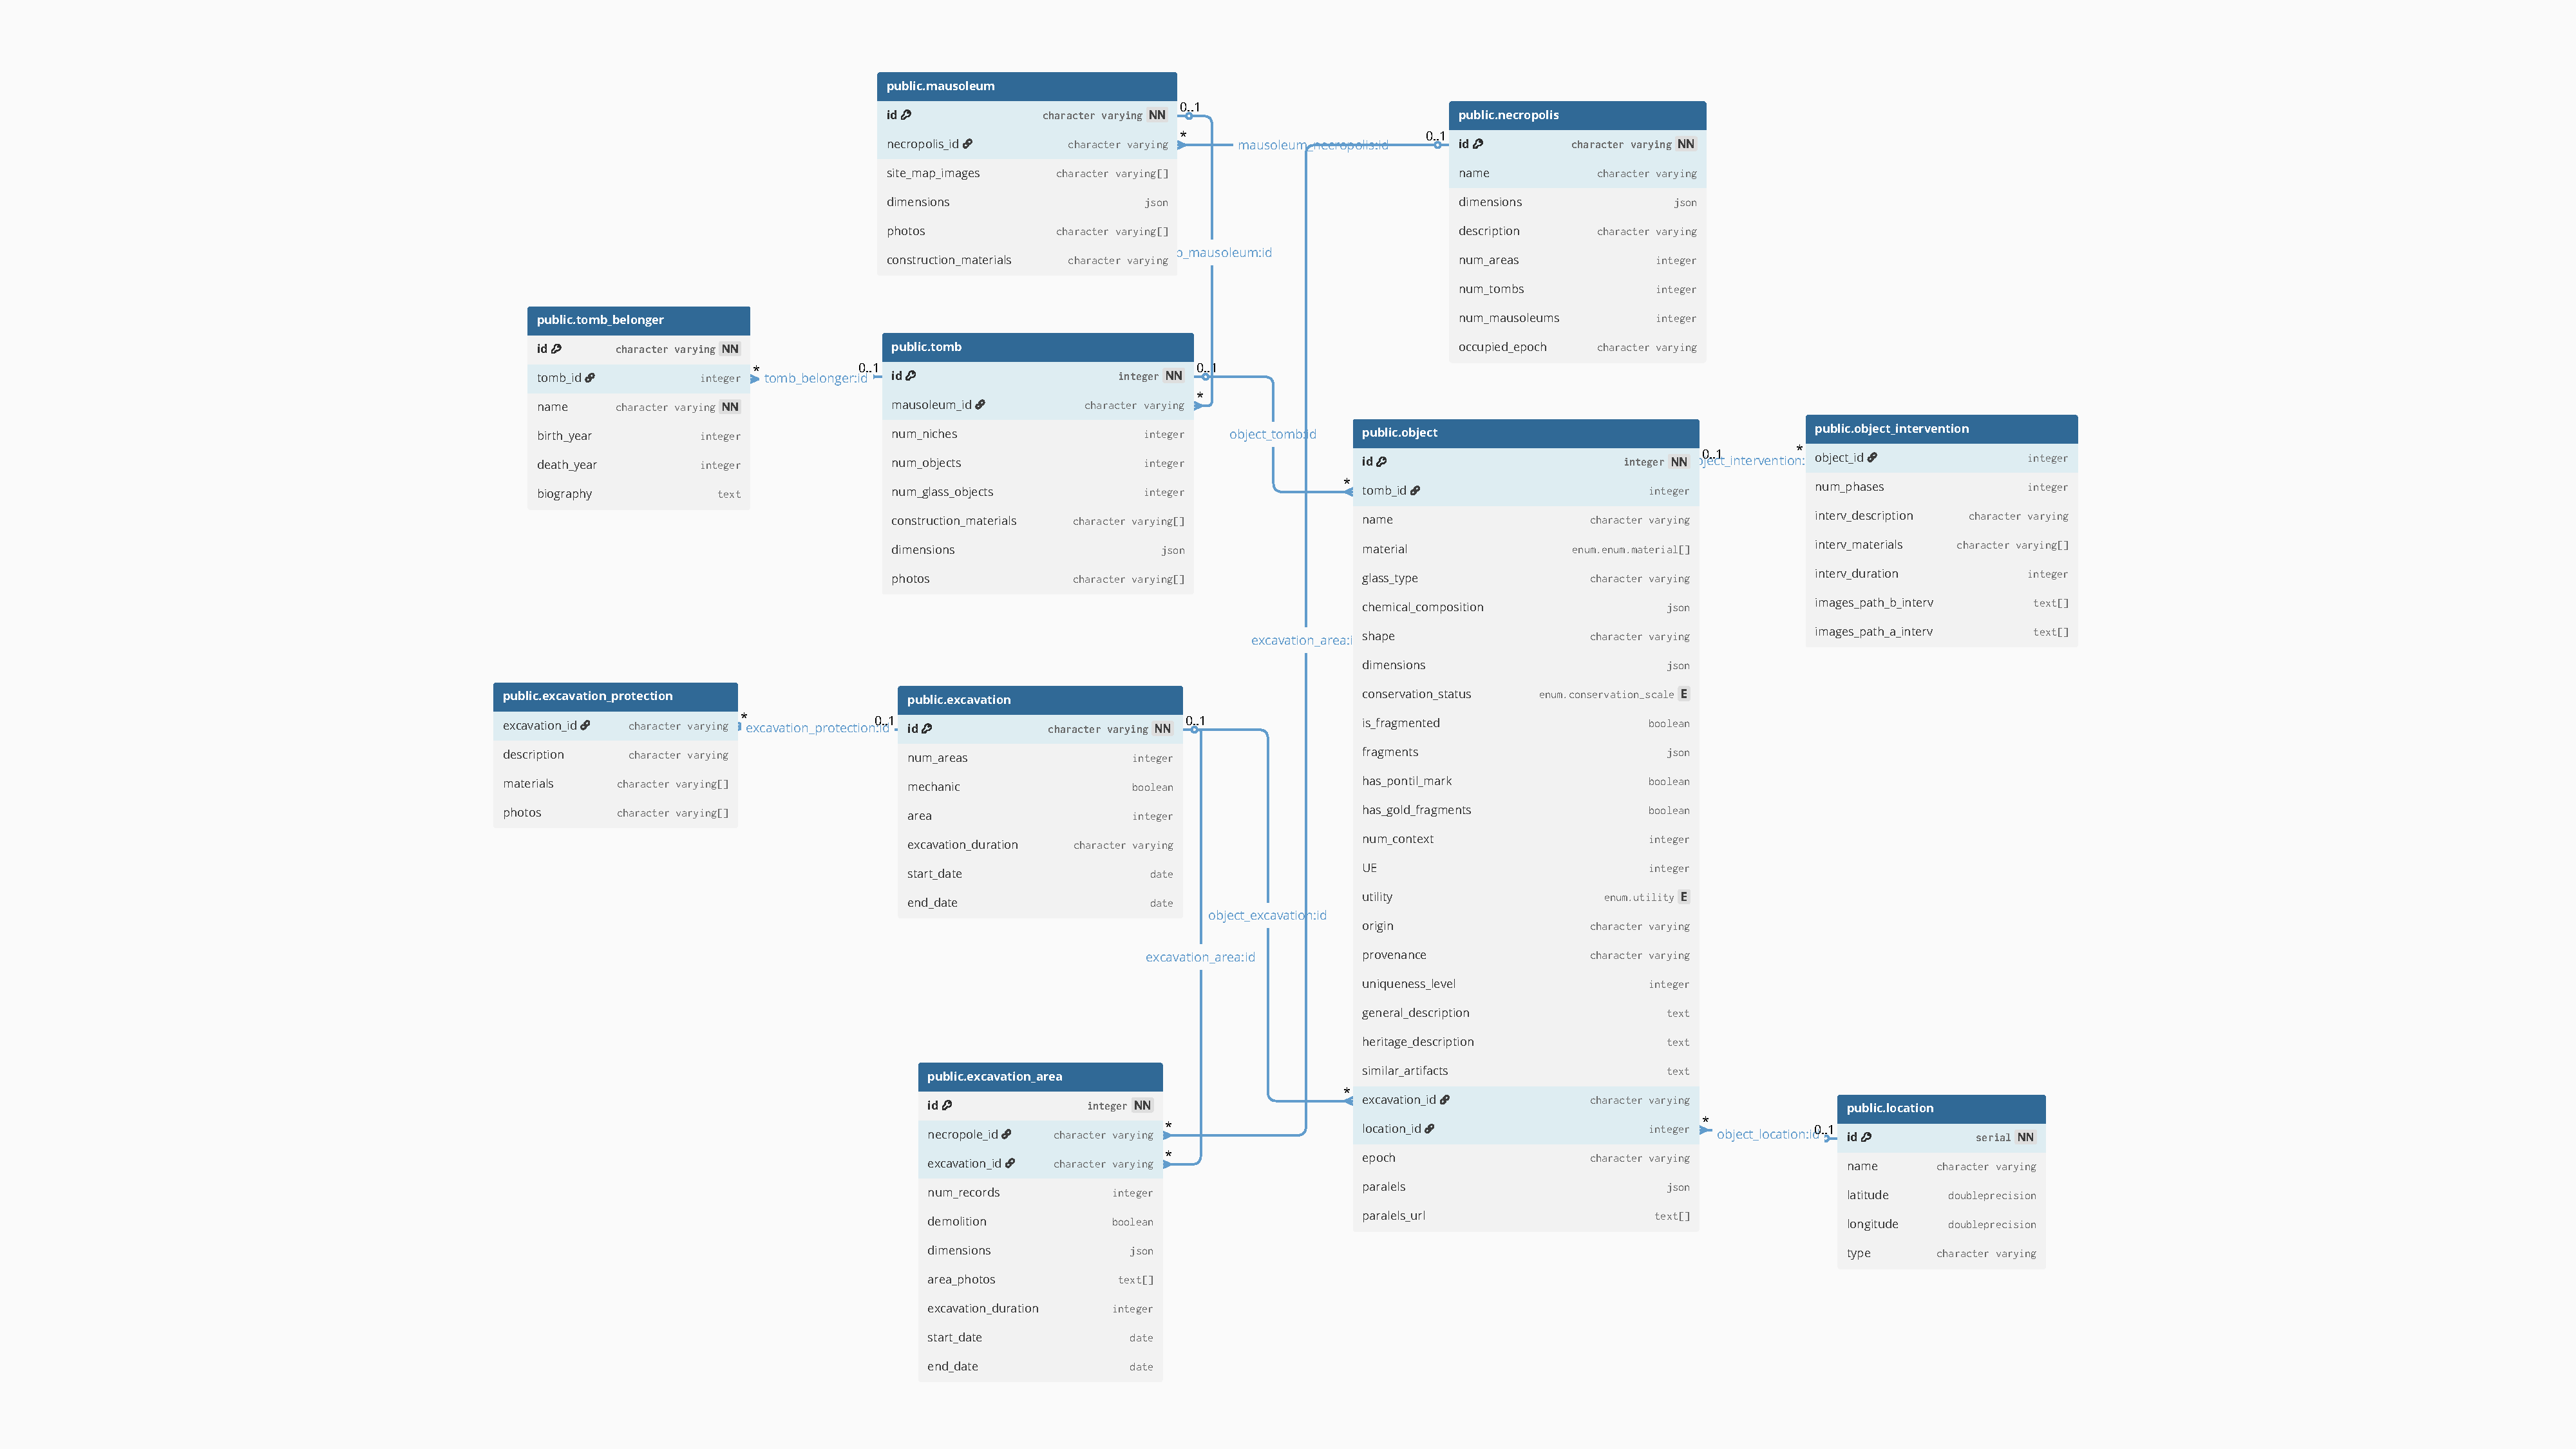
\includegraphics[width=1\linewidth, trim=10cm 0cm 10cm 0cm, clip]{thesis_db_}
    \caption{Relational Database Model.} 
    \label{fig:database}
\end{figure}


The database model was designed considering future extensibility. Initially, it was structured to store significant data from the necropolis, including the funerary enclosure and tomb under study. The structure was generalized to improve scalability, flexibility to possibly include data, such as other tombs, associated objects, and aggregate the maximum information. 
Throughout the thesis period, the database structure was continuously refined and restructured with new tables, relations, and data fields.

It was decided to not store the entire image, as binary data in the database. Instead, only file paths to the images were saved. This allowed for efficient access and manipulation of images, while other object-related data, such as text and links, was fully stored in the database.

For generating the data model, SQL was used to create a database dump.
Using "dbdiagram.io", this dump was translated into a visual diagram showing tables and their relations. This tool streamlined the creation of the Entity-Relationship diagram through code.


\section{Design Choices}
\label{sec:design}
Initially, the idea involved creating a map using JavaScript and its Leaflet.js\footnote{\url{https://leafletjs.com/}} library. 
However, the dissertation's direction shifted towards integrating the map with the funerary enclosure and its elements directly in Unity, forming a unified \gls{VE}. This way, the users can walk across the map as if in reality, while simultaneously viewing the \gls{3D} model accurately positioned in space. 
The map itself still holds potential for further enhancement, which could contribute to a more complete and immersive experience within the \gls{VE}.

%Incluo seccao de dificuldades/desafios ao lonbgo do desenvolvimento? 
%ou vou colocando na seccao pretendzida;;ex: hand tracking vs controllers


% \chapter{Proposed Work}
% \label{cha:proposed_work}

% This chapter aims to outline the approach that will be used to achieve the project objectives defined in Chapter \ref{cha:introduction}, while providing the prior work in the various areas relevant to this study.

% \section{Requirements}
% \label{sec:requirements}

% This section describes the requirements and functionalities to be developed during this dissertation, categorized into the following areas: Interactive Map, \gls{3D} Model Interaction, Repository, and \gls{VR} environment.

% Given the diverse requirements of this project, the primary focus will be on developing an immersive \gls{VE}, prioritizing \gls{3D} models and \gls{VR} for exploring glass artifacts within the tomb. The interactive map features will be included but may be implemented with less detail.

% \subsection*{Interactive Map}
% A map of the Troia archaeological site under study will be incorporated into the project to offer interactive functionalities.
% \begin{itemize}
%     \item \textbf{Map Zoom \& Navigation:} Users can pan, zoom, and explore different locations.
%     \item \textbf{Perspective Switching:} Toggle between top-down and profile views for better spatial understanding.
%     \item \textbf{Geospatial Data Integration:} Include \gls{GIS} layers combining excavation findings, and overlay a \textit{.tif} map illustration with some immersive interaction.
%     \item \textbf{Layer Toggle:} Toggle visibility of layers, such as excavation campaigns or glass antiquities.
%     \item \textbf{Parallel Objects:} Link parallel excavation findings/museums, possibly integrating them in the object pop-up on the map.
% \end{itemize}

% \subsection*{\gls{3D} Models \& Interaction}
% A dedicated component will focus on the interaction with \gls{3D} models, which will later be integrated into a \gls{VR} environment.
% \begin{itemize}
%     \item \textbf{Artifact Interaction:} Allows users to virtually manipulate (rotate, zoom etc) the glass artefact models, as well as apply different textures.
%     \item \textbf{Contextual Overlay:} Display descriptive metadata about the artefact, such as its origin, period, and historical usage.
%     \item \textbf{Reconstructed Models:} Showcase how artefacts would look originally (having in consideration characteristics such as: colourless glass, archaeological drawings and symmetry). However, due to time constraints and the need to model the original artefacts, the reconstruction functionality may not be completed.
%     \item \textbf{3D Models Integration:} The user can zoom the map to visualize the perspective of a specific \gls{3D} model.
%     %select a position to visualize the perspective of their 3D model.
% \end{itemize}

% \subsection*{Repository}
% The repository will consist of a spatial database designed to store and manage data from the mausoleum under study.
% \begin{itemize}
%     \item \textbf{Document Upload/Download:} Allow contributors to upload images, videos or excavation reports of the archaeological intervention.
%     \item \textbf{Search and Filter Features:} Users can search and filter based on some fields, such as time period, shape, and provenance.
%     \item \textbf{Digital Preservation:} The usage of open, and standard formats to ensure a long-term resource access.
% \end{itemize}


% \subsection*{\gls{VR} Environment}
% \gls{VR} functionalities will provide an intuitive user experience, enabling interaction with the \gls{VE} through the use of \glspl{HMD}.
% \begin{itemize}
%     \item \textbf{Immersive Experience:} \gls{VR} allows users to immerse in a virtual tomb visit, enabling interaction with glass relics.
%     \item \textbf{Device Accessibility:} Primarily user-friendly and enabling haptic interaction, while supporting \gls{VR} glasses as an emerging display option.
%     \item \textbf{Localization \& Wayfinding:} 
%     \begin{itemize}
%         \item \textbf{\gls{POI}:} Use colors, text, visual markers, or direction arrows to emphasize and guide users to historically significant locations.
%     \end{itemize}
%    % \item \textbf{Multilingual Support:} Provide language options to ensure accessibility for an international audience.
% \end{itemize}

% \section{Development Technologies and Tools}
% \label{sec:technologies}

% The following section focuses on the technologies and tools that will be used in the implementation of this project. These include frontend, backend, database, and \gls{3D} development tools.

% \subsection{Web Mapping Development}

% \subsubsection{Frontend Technologies}
% \label{sec:frontend}

% JavaScript is a programming language mostly used to control interactive behavior in web
% pages. To make a map interactive, most websites automatically send JavaScript code to the browser~\cite{ajayi2024utilizing}. In this project, this language will be used for client-side web development and to integrate frameworks that enhance map interactivity.

% Leaflet\footnote{\url{https://leafletjs.com/}} is an open-source JavaScript library that facilitates the creation of mobile-friendly interactive maps. It offers a wide array of plugins that improve usability and simplify application development.
% Leaflet will be employed in this thesis to integrate interactive map features and create an intuitive user interface.

% Other alternatives for web development frameworks used for map rendering and interaction include OpenLayers\footnote{\url{https://openlayers.org/}}, which enables the integration of dynamic maps into web pages and can display map tiles, vector data, and markers loaded from any source.
% Another powerful tool is the Google Maps API\footnote{\url{https://developers.google.com/maps}}, which allows developers to embed Google Maps functionalities directly into both web and mobile applications.
% Additionally, Mapbox\footnote{\url{https://www.mapbox.com/}} and \gls{OSM}\footnote{\url{https://www.openstreetmap.org/}} provide online mapping solutions. While \gls{OSM} is open-source, offering greater flexibility and customization, and is maintained and updated by the community, Mapbox and Google Maps API have usage-based pricing plans.
% For this dissertation, one of these technologies will be used to create an interactive map, complementing an existing illustration of the Troia site area, that includes the mausoleum under study. This will be supplemented with an open map, potentially sourced from \gls{OSM}\footnote{\url{https://www.openstreetmap.org/}}.

% \subsubsection{Backend Technologies}
% \label{sec:backend} 

% The backend technology selected for this thesis is Node.js, an open-source, cross-platform JavaScript runtime environment. Node.js enables developers to create servers, web applications, command-line tools, and automation programs.

% In this project, Node.js will be used to support the web server and to improve performance and scalability when handling repository data. Additionally, it will streamline the communication between the backend and the database repository.


% \subsection{Unity Engine}
% \label{sec:unity_description} 

% Unity is a cross-platform engine that provides a robust environment for developing \gls{2D} and \gls{3D} applications. 
% Its component-based architecture simplifies \gls{3D} development by allowing developers to define object behaviors through scripts in \glspl{VE}.
% Despite not being open-source, Unity offers a community forum and repositories where developers can access resources, and adapt them for their projects.
% Additionally, the Unity Learn\footnote{\url{https://learn.unity.com/}} platform provides free tutorials, simplifying the learning process.

% Unity will be a fundamental technology for supporting the \gls{VR} development of this project. Its integration enables users an immersive experience by visualizing several \gls{3D} data types, including excavation and glass artefacts metadata. 
% Additionally, C\# programming language within Unity facilitates the management of game objects and user interactions in the \gls{VE}.


% \subsection{Database Repository}
% \label{sec:repos}

% There are several alternatives for storage management systems, but the options are more limited when it comes to geographical
% database systems.

% For this project, organizing the data in a relational database is more appropriate due to its flexibility and consistency.
% The most common databases for such applications include PostGIS, extension for PostgreSQL, MySQL\footnote{\url{https://www.mysql.com/}} and Oracle.
% All three databases databases support spatial data types, allowing to store and manage geographic objects, representing them with points, lines, or polygons, and performing geospatial queries.
% Among these, PostGIS is widely used for spatial data storage, geometry processing, and efficient geospatial querying.
% Oracle supports advanced spatial features and 3D features but has a commercial license. On the other hand, MySQL is open-source and more suitable for small-to-medium-scale projects.

% PostgreSQL database was chosen for this thesis because of its high performance and flexibility in managing spatial data. All geographic data, artefacts metadata, and excavation details will be stored within this system.


% \subsection{Photogrammetry Tools}
% \label{sec:photogrammetry_tool} 

% The software that will be used to process digital images and generate \gls{3D} object models is \textit{Agisoft Metashape}\footnote{\url{https://www.agisoft.com/}}.
% This software performs photogrammetric processing of digital images to generate \gls{3D} spatial data, which can be applied in various fields such as \gls{GIS} applications, \gls{CH} documentation, visual effects production, and indirect measurements of objects of diverse scales. 
% By stitching together photographs, \textit{Agisoft Metashape} captures the geometry, texture, and visual appearance of physical objects or environments.
% Other alternatives for photogrammetry softwares are Pix4D\footnote{\url{https://www.pix4d.com/}}, RealityCapture\footnote{\url{https://www.capturingreality.com/}} and DroneDeploy\footnote{\url{https://www.dronedeploy.com/}}

% There are some already built models of the artefacts provided by Troia archaeologists, there will be done a selection and evaluation of the greatest possibilities.


% \section{System Architecture}
% \label{sec:architecture}

% This section includes an overview of the system architecture. The communication flow between the layers will be conducted by a REST \gls{API}.
% REST \glspl{API} with Node.js connects components in microservices architectures\footnote{\url{https://www.ibm.com/think/topics/rest-apis}}.
% This service was selected due to its flexibility and lightweight solution. 

% \begin{figure}[h!]
% \centering
% 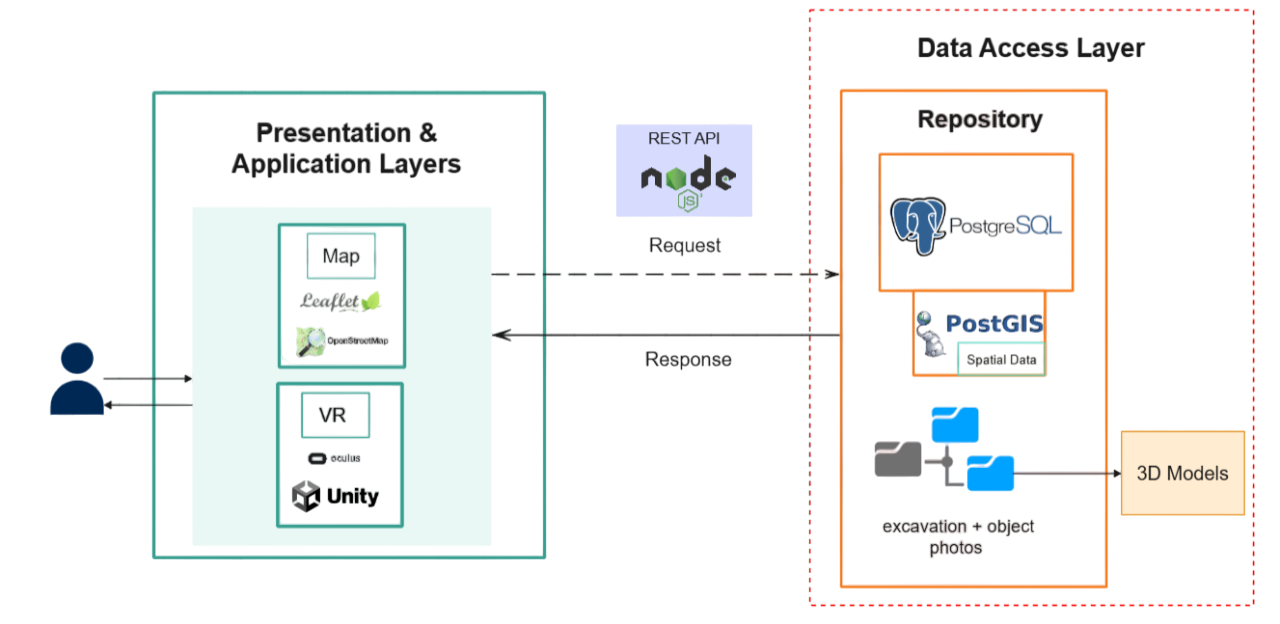
\includegraphics[width=1.0\linewidth]{system_architecture2}
% \caption{System Architecture Overview}
% \label{fig:architecture}
% \end{figure}
% \FloatBarrier

% \section{Usability Tests}
% \label{sec:usability_tests}

% The Usability Tests will be conducted both remotely and presencially throughout the implementation process, specifically the \gls{HMD} interactions will be done in person.
% Investigators from \gls{VICARTE} will participate in these tests with valuable feedback to improve the platform, while providing input on their archeology necessities. Their collaboration will contribute to a more useful, accurate, and user-friendly platform.

% \section{Previous Work}
% \label{sec:previous_work}

% During the curricular internship, a platform was developed using React\footnote{\url{https://react.dev/}} and TailwindCSS for the web layer, with C\# and ASP.NET for the application layer, and MongoDB\footnote{\url{https://www.mongodb.com/}} for data storage. Communication between these three components was handled through direct requests to the web server, which forwarded \gls{CRUD} operations and interacted with the database.  
% Additionally, the Database Systems and Cloud Computation Systems master's course provided hands-on experience in various storage methodologies and introduced different technologies and alternative solutions for data management.

% This section explains the various experiments carried out during the preparation phase.

% \subsection{Web \gls{GIS}}
% \label{sec:gis_previous} 

% To further develop expertise in \gls{GIS}, enrollment was made in the master's GeoWeb course taught by the thesis adviser, Armanda Rodrigues. During this course, was developed a Web \gls{3D} application designed to provide an interactive map for visualizing and analyzing demographic data, key infrastructure locations, and other notable European datasets. Although this project did not focus on archaeological data, it introduced and enriched the understanding of GIS concepts, map interaction, and geospatial analysis while exposing new technologies.

% The application leveraged PostGIS, a PostgreSQL extension that supports spatial operations.
% Additionally, frameworks like Leaflet were used for map rendering, visualization, and user interaction. For the base map, \gls{OSM} was integrated, offering a customizable and versatile visualization. This project serves as a preparatory stage for my thesis, specifically for the \gls{GIS} component, in which I will develop an interactive map of the Troia site.

% \section{Data Structure Proposal}
% \label{sec:data_strucutre}

% A preliminary database structure has been proposed and analysed for artefacts storage management.  
% It incorporates the key characteristics of each object to ensure structured organization and availability.

% \begin{figure}[h!]
%     \centering
%     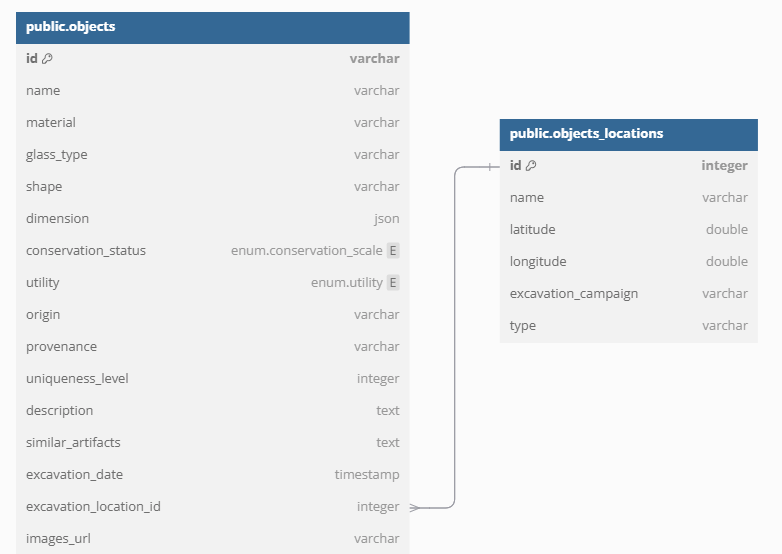
\includegraphics[width=0.7\textwidth]{data_structure}
%     \caption{Proposed Data Structure for Managing Artifacts Data.}
%     \label{fig:data_strucutre}
% \end{figure}
% \FloatBarrier

% \subsection{Photogrammetry}
% \label{sec:photogrammetry_previous} 

% During the preparation, a photogrammetric experiment was conducted by the student using the \textit{Agisoft Metashape} environment. A total of 143 images were collected during the excavation campaign by the restoration department of NOVA for analysis. 
% Based on these images, a \gls{3D} model was generated from the photogrammetric survey and subsequently imported into the \textit{Sketchfab} viewer for intuitive interaction.
% Within the grave where the deceased was buried, three open triangular areas were identified, containing the precious artefacts of the defunct, as shown in Figure~\ref{fig:model3} below.

% \begin{figure}[h!]
%     \centering
%     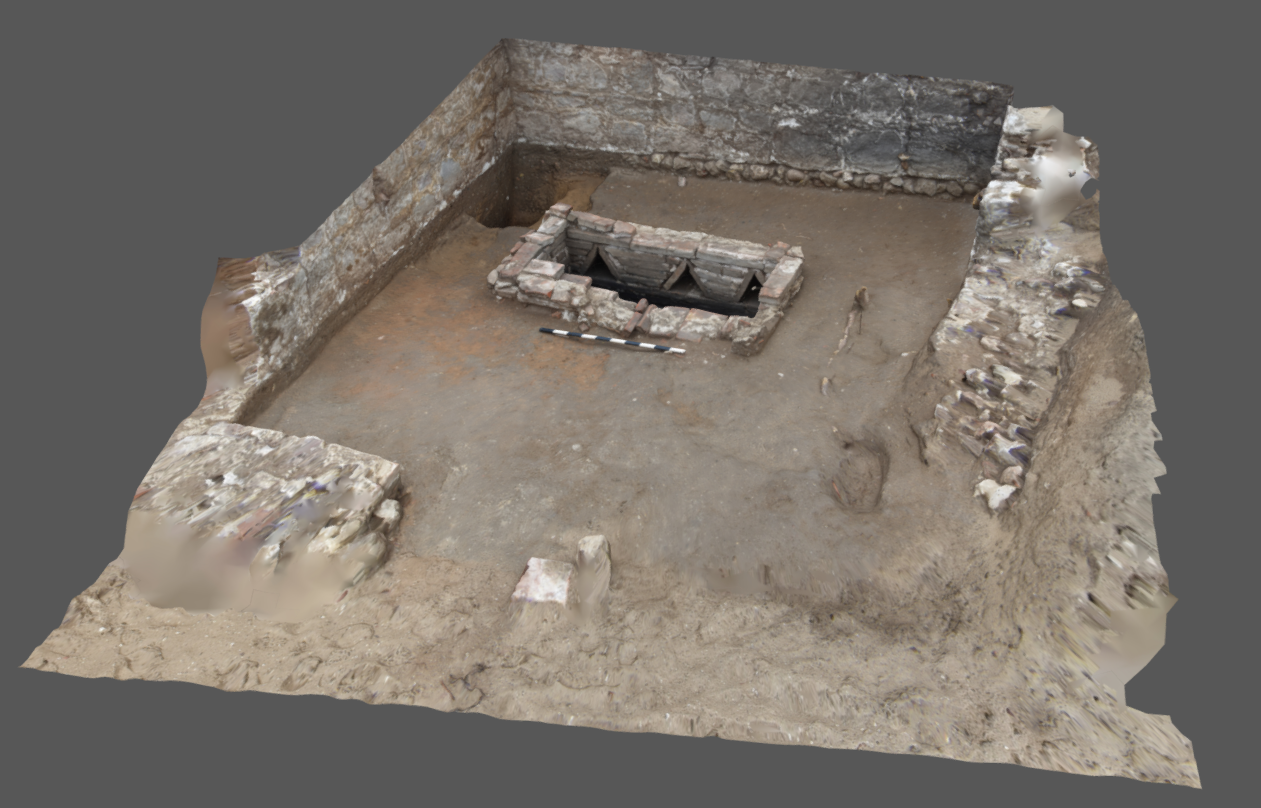
\includegraphics[width=0.7\textwidth]{model3}
%     \caption{\gls{3D} Model Imported into Sketchfab for Visualization.}
%     \label{fig:model3}
% \end{figure}
% \FloatBarrier

% \subsection{Unity}
% \label{sec:unity} 

% To reproduce the visualization of the \gls{3D} models on the map, a simulation was created in Unity, as presented in Figure \ref{fig:overlay}. The goal was to overlay the map with the \gls{3D} excavation model.
% To achieve this, the illustrated map was placed as the ground surface, with the excavation model positioned above it. The ultimate objective is to apply this approach to the artefacts found within the three triangular areas of the grave.

% This experiment simulates an intended interactive and dynamic experience, allowing users to explore the map and objects through interactive layers while using an \gls{HMD}.

% \begin{figure}[h!]
%     \centering
%     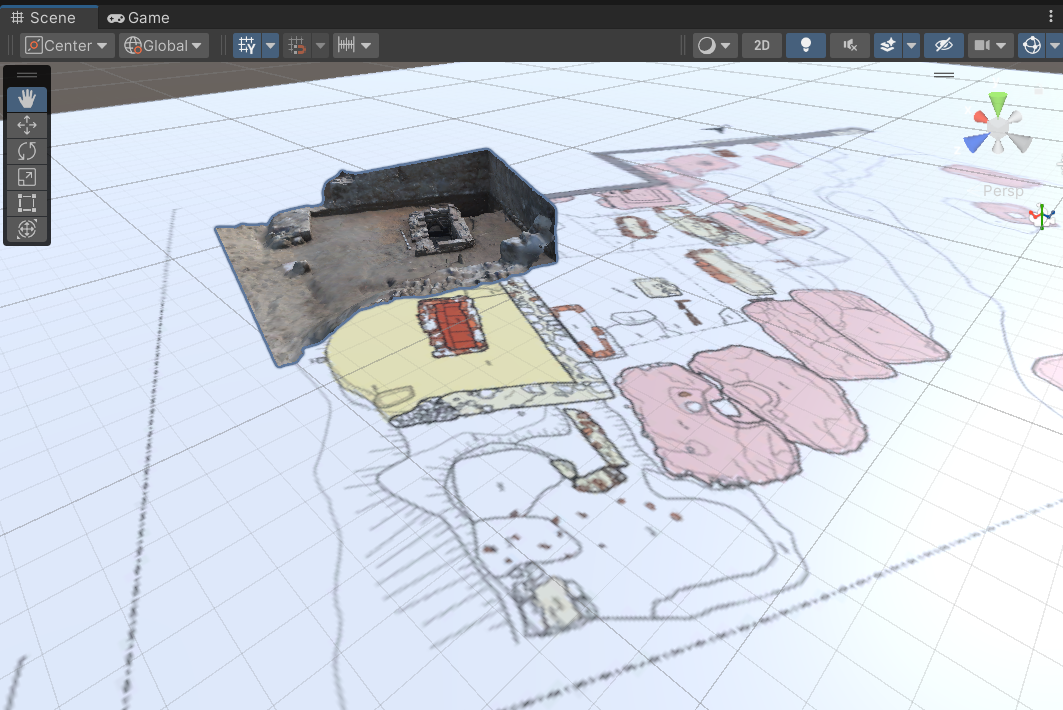
\includegraphics[width=0.7\textwidth]{overlay_test}
%     \caption{Overlay \gls{3D} Excavation Model with a Map Representation.}
%     \label{fig:overlay}
% \end{figure}
% \FloatBarrier


% \section{Work Plan}
% \label{cha:work_plan}

% This section contains the planned progress, organized into distinct tasks, each with a description. Some tasks will be developed in parallel. 
% Additionally, a Gantt chart is presented in Figure \ref{fig:gantt_chart} to illustrate the timeline for each task.

% \begin{itemize}
%     \item \textbf{Mockup Development}: This task focuses on developing a mockup that includes map visualization within a \gls{VE}, along with the associated functionalities and \gls{3D} models visualization.
%     \item \textbf{\gls{VE} Development}: This phase involves creating an immersive environment where users can navigate, and select objects, followed by the implementation of interactive functionalities with \gls{3D} models of the artefacts. These interactions include applying filters, zooming, and scaling. Initially, the development will focus on a simulation with a single object.
%     \item \textbf{\gls{GIS} Implementation}: This task comprises the creation of a map that allows user interaction with \gls{POI} represented by markers, integrating layers, and providing functionalities as outlined in Section \ref{sec:requirements}. Although the \gls{GIS} and \gls{VR} tools are developed in parallel, it may be possible to transfer from the map to the immersive environment through user interaction (e.g., clicking on a location on the map to display its \gls{3D} model), or the other way around.
%     \item \textbf{Database Creation for Repository}: In this phase, a database will be established to store significant data, including artefact and excavation metadata. The structure will initially focus on a single object, as proposed in Section \ref{sec:data_strucutre}. The database will be continuously updated over several weeks to data loading and modifications.
%     \item \textbf{System Evaluation \& Testing}: This task involves testing functionalities, usability, and performance, with participation from VICARTE investigators. Following the conclusion of the testing phase, the system evaluation process will begin with user questionnaires, leading to potential improvements based on the feedback received.  
%     \item \textbf{Documentation}: The dissertation report will be developed during the whole process.
% \end{itemize}

% % \begin{figure}[h!]
% %     \centering
% %     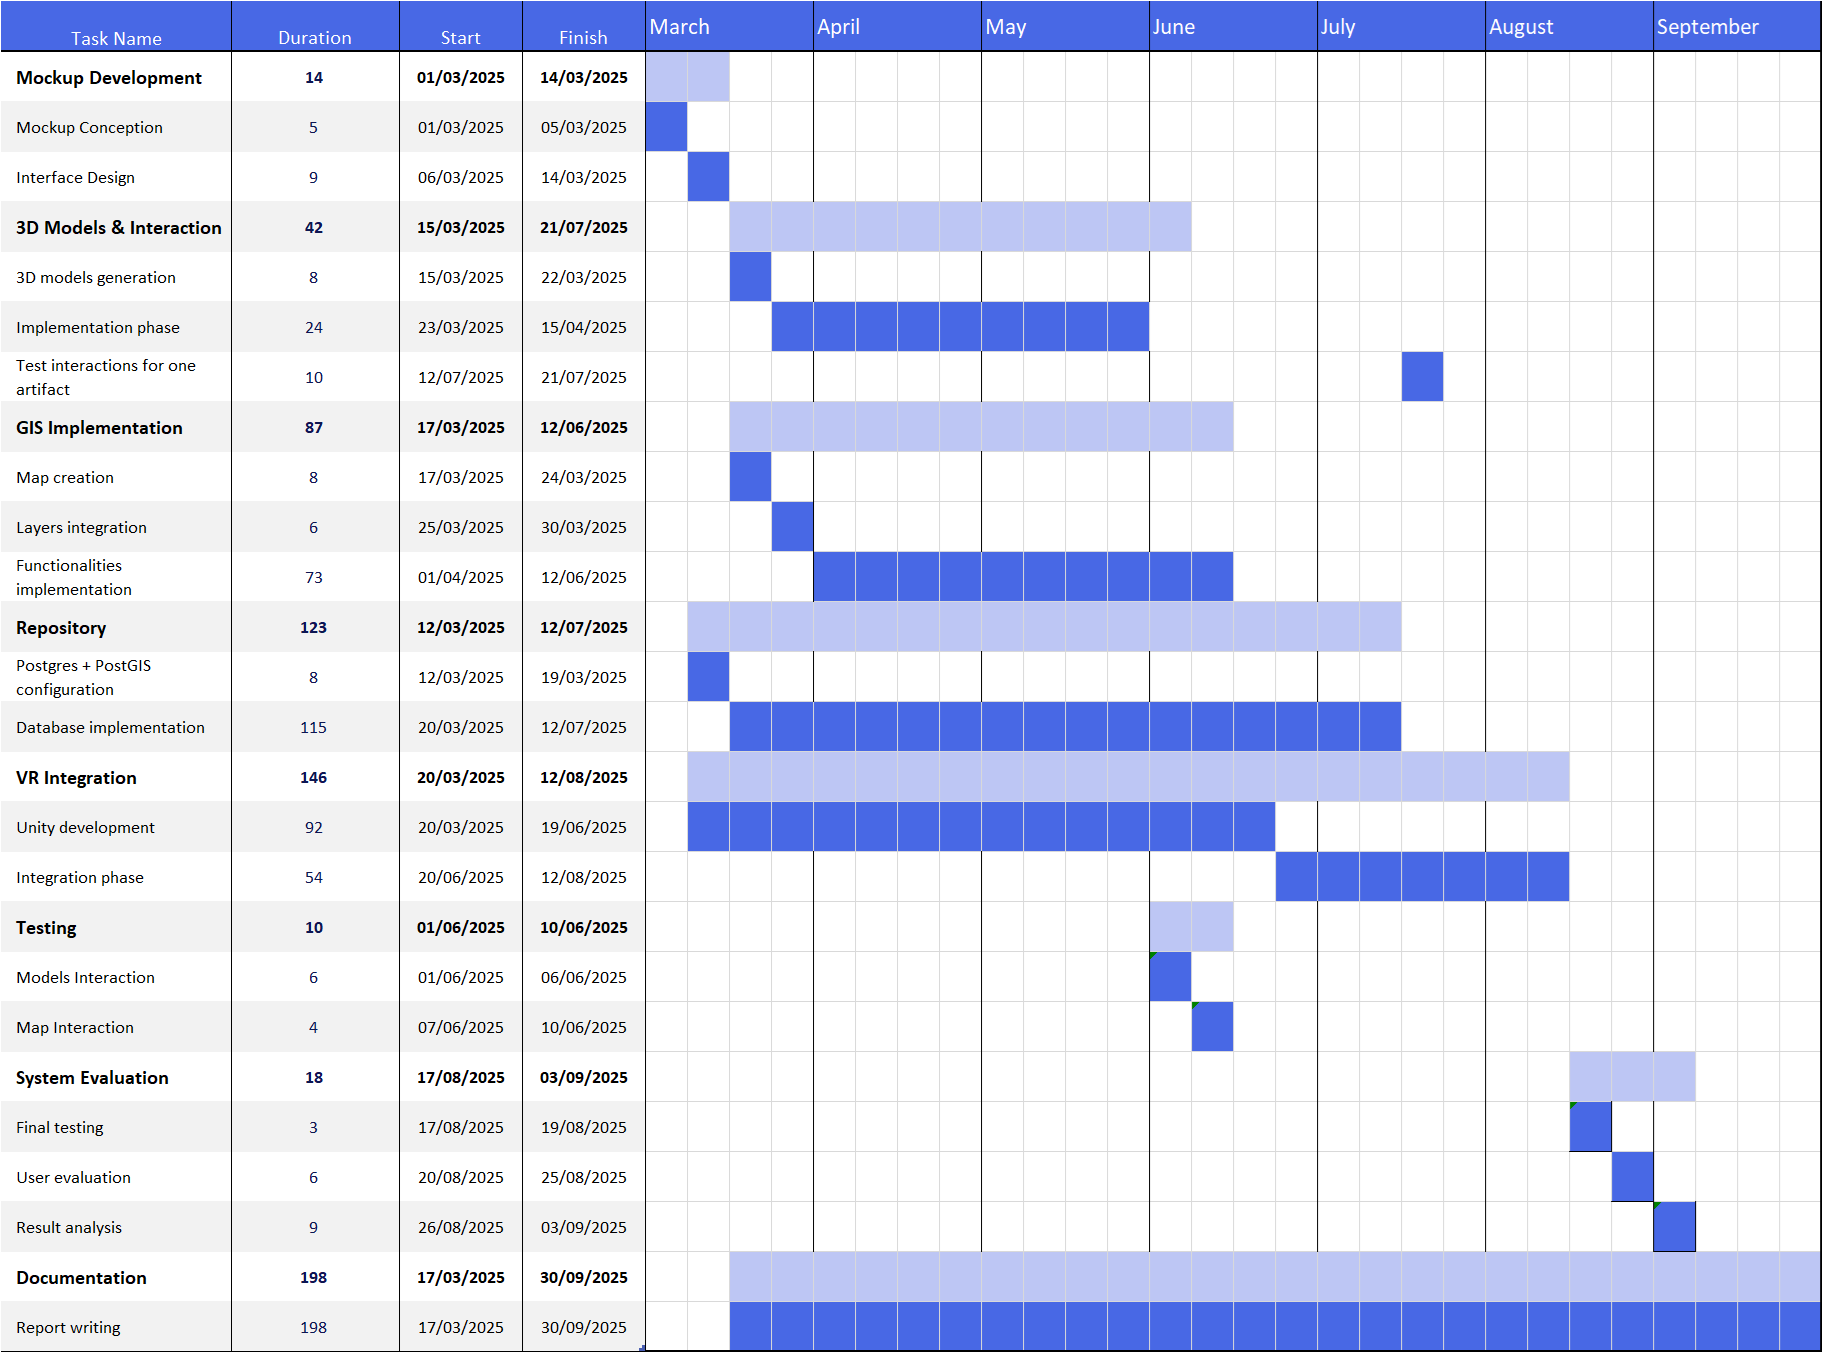
\includegraphics[width=1.0\linewidth]{Gantt_chart}
% %     \caption{Gantt Chart Representation of the Work Plan.}
% %     \label{fig:gantt_chart}
% %   \end{figure}
% %   \FloatBarrier


% %   \begin{figure}[h!]
% %     \centering
% %     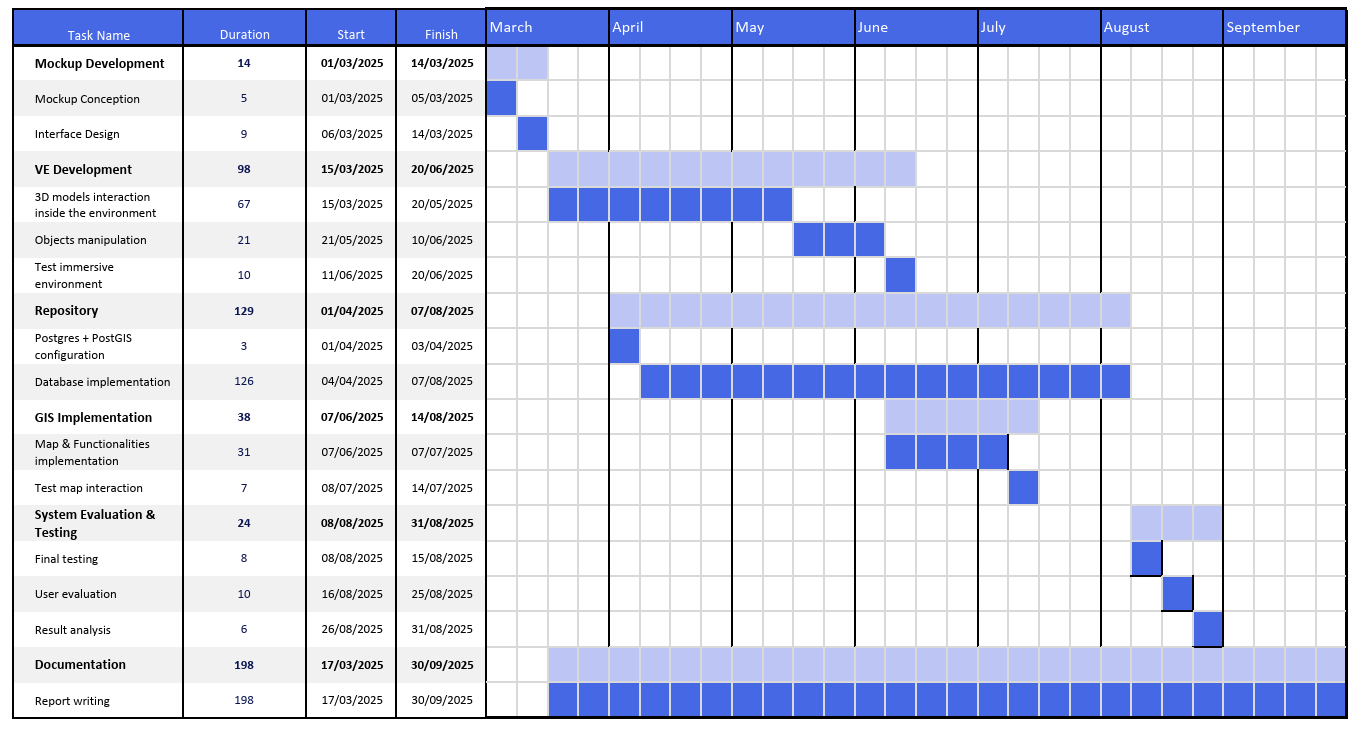
\includegraphics[width=1.0\linewidth]{gantt_chartt}
% %     \caption{Gantt Chart Representation of the Work Plan.}
% %     \label{fig:gantt_chart}
% %   \end{figure}
% %   \FloatBarrier

%   \begin{figure}[h!]
%     \centering
%     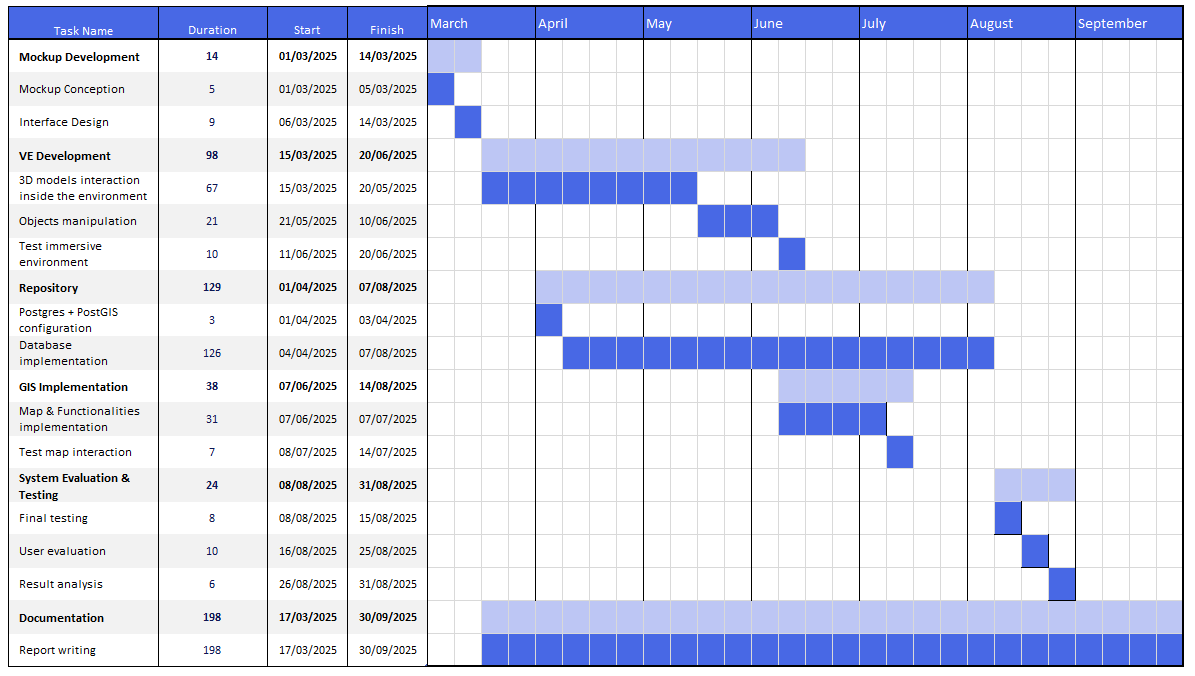
\includegraphics[width=1.0\linewidth]{gantt_chartt2}
%     \caption{Gantt Chart Representation of the Work Plan.}
%     \label{fig:gantt_chart}
%   \end{figure}
%   \FloatBarrier


%Incluo seccao de dificuldades/desafios ao lonbgo do desenvolvimento? 
%ou vou colocando na seccao pretendzida;;ex: hand tracking vs controllers


% \chapter{Proposed Work}
% \label{cha:proposed_work}

% This chapter aims to outline the approach that will be used to achieve the project objectives defined in Chapter \ref{cha:introduction}, while providing the prior work in the various areas relevant to this study.

% \section{Requirements}
% \label{sec:requirements}

% This section describes the requirements and functionalities to be developed during this dissertation, categorized into the following areas: Interactive Map, \gls{3D} Model Interaction, Repository, and \gls{VR} environment.

% Given the diverse requirements of this project, the primary focus will be on developing an immersive \gls{VE}, prioritizing \gls{3D} models and \gls{VR} for exploring glass artifacts within the tomb. The interactive map features will be included but may be implemented with less detail.

% \subsection*{Interactive Map}
% A map of the Troia archaeological site under study will be incorporated into the project to offer interactive functionalities.
% \begin{itemize}
%     \item \textbf{Map Zoom \& Navigation:} Users can pan, zoom, and explore different locations.
%     \item \textbf{Perspective Switching:} Toggle between top-down and profile views for better spatial understanding.
%     \item \textbf{Geospatial Data Integration:} Include \gls{GIS} layers combining excavation findings, and overlay a \textit{.tif} map illustration with some immersive interaction.
%     \item \textbf{Layer Toggle:} Toggle visibility of layers, such as excavation campaigns or glass antiquities.
%     \item \textbf{Parallel Objects:} Link parallel excavation findings/museums, possibly integrating them in the object pop-up on the map.
% \end{itemize}

% \subsection*{\gls{3D} Models \& Interaction}
% A dedicated component will focus on the interaction with \gls{3D} models, which will later be integrated into a \gls{VR} environment.
% \begin{itemize}
%     \item \textbf{Artifact Interaction:} Allows users to virtually manipulate (rotate, zoom etc) the glass artefact models, as well as apply different textures.
%     \item \textbf{Contextual Overlay:} Display descriptive metadata about the artefact, such as its origin, period, and historical usage.
%     \item \textbf{Reconstructed Models:} Showcase how artefacts would look originally (having in consideration characteristics such as: colourless glass, archaeological drawings and symmetry). However, due to time constraints and the need to model the original artefacts, the reconstruction functionality may not be completed.
%     \item \textbf{3D Models Integration:} The user can zoom the map to visualize the perspective of a specific \gls{3D} model.
%     %select a position to visualize the perspective of their 3D model.
% \end{itemize}

% \subsection*{Repository}
% The repository will consist of a spatial database designed to store and manage data from the mausoleum under study.
% \begin{itemize}
%     \item \textbf{Document Upload/Download:} Allow contributors to upload images, videos or excavation reports of the archaeological intervention.
%     \item \textbf{Search and Filter Features:} Users can search and filter based on some fields, such as time period, shape, and provenance.
%     \item \textbf{Digital Preservation:} The usage of open, and standard formats to ensure a long-term resource access.
% \end{itemize}


% \subsection*{\gls{VR} Environment}
% \gls{VR} functionalities will provide an intuitive user experience, enabling interaction with the \gls{VE} through the use of \glspl{HMD}.
% \begin{itemize}
%     \item \textbf{Immersive Experience:} \gls{VR} allows users to immerse in a virtual tomb visit, enabling interaction with glass relics.
%     \item \textbf{Device Accessibility:} Primarily user-friendly and enabling haptic interaction, while supporting \gls{VR} glasses as an emerging display option.
%     \item \textbf{Localization \& Wayfinding:} 
%     \begin{itemize}
%         \item \textbf{\gls{POI}:} Use colors, text, visual markers, or direction arrows to emphasize and guide users to historically significant locations.
%     \end{itemize}
%    % \item \textbf{Multilingual Support:} Provide language options to ensure accessibility for an international audience.
% \end{itemize}

% \section{Development Technologies and Tools}
% \label{sec:technologies}

% The following section focuses on the technologies and tools that will be used in the implementation of this project. These include frontend, backend, database, and \gls{3D} development tools.

% \subsection{Web Mapping Development}

% \subsubsection{Frontend Technologies}
% \label{sec:frontend}

% JavaScript is a programming language mostly used to control interactive behavior in web
% pages. To make a map interactive, most websites automatically send JavaScript code to the browser~\cite{ajayi2024utilizing}. In this project, this language will be used for client-side web development and to integrate frameworks that enhance map interactivity.

% Leaflet\footnote{\url{https://leafletjs.com/}} is an open-source JavaScript library that facilitates the creation of mobile-friendly interactive maps. It offers a wide array of plugins that improve usability and simplify application development.
% Leaflet will be employed in this thesis to integrate interactive map features and create an intuitive user interface.

% Other alternatives for web development frameworks used for map rendering and interaction include OpenLayers\footnote{\url{https://openlayers.org/}}, which enables the integration of dynamic maps into web pages and can display map tiles, vector data, and markers loaded from any source.
% Another powerful tool is the Google Maps API\footnote{\url{https://developers.google.com/maps}}, which allows developers to embed Google Maps functionalities directly into both web and mobile applications.
% Additionally, Mapbox\footnote{\url{https://www.mapbox.com/}} and \gls{OSM}\footnote{\url{https://www.openstreetmap.org/}} provide online mapping solutions. While \gls{OSM} is open-source, offering greater flexibility and customization, and is maintained and updated by the community, Mapbox and Google Maps API have usage-based pricing plans.
% For this dissertation, one of these technologies will be used to create an interactive map, complementing an existing illustration of the Troia site area, that includes the mausoleum under study. This will be supplemented with an open map, potentially sourced from \gls{OSM}\footnote{\url{https://www.openstreetmap.org/}}.

% \subsubsection{Backend Technologies}
% \label{sec:backend} 

% The backend technology selected for this thesis is Node.js, an open-source, cross-platform JavaScript runtime environment. Node.js enables developers to create servers, web applications, command-line tools, and automation programs.

% In this project, Node.js will be used to support the web server and to improve performance and scalability when handling repository data. Additionally, it will streamline the communication between the backend and the database repository.


% \subsection{Unity Engine}
% \label{sec:unity_description} 

% Unity is a cross-platform engine that provides a robust environment for developing \gls{2D} and \gls{3D} applications. 
% Its component-based architecture simplifies \gls{3D} development by allowing developers to define object behaviors through scripts in \glspl{VE}.
% Despite not being open-source, Unity offers a community forum and repositories where developers can access resources, and adapt them for their projects.
% Additionally, the Unity Learn\footnote{\url{https://learn.unity.com/}} platform provides free tutorials, simplifying the learning process.

% Unity will be a fundamental technology for supporting the \gls{VR} development of this project. Its integration enables users an immersive experience by visualizing several \gls{3D} data types, including excavation and glass artefacts metadata. 
% Additionally, C\# programming language within Unity facilitates the management of game objects and user interactions in the \gls{VE}.


% \subsection{Database Repository}
% \label{sec:repos}

% There are several alternatives for storage management systems, but the options are more limited when it comes to geographical
% database systems.

% For this project, organizing the data in a relational database is more appropriate due to its flexibility and consistency.
% The most common databases for such applications include PostGIS, extension for PostgreSQL, MySQL\footnote{\url{https://www.mysql.com/}} and Oracle.
% All three databases databases support spatial data types, allowing to store and manage geographic objects, representing them with points, lines, or polygons, and performing geospatial queries.
% Among these, PostGIS is widely used for spatial data storage, geometry processing, and efficient geospatial querying.
% Oracle supports advanced spatial features and 3D features but has a commercial license. On the other hand, MySQL is open-source and more suitable for small-to-medium-scale projects.

% PostgreSQL database was chosen for this thesis because of its high performance and flexibility in managing spatial data. All geographic data, artefacts metadata, and excavation details will be stored within this system.


% \subsection{Photogrammetry Tools}
% \label{sec:photogrammetry_tool} 

% The software that will be used to process digital images and generate \gls{3D} object models is \textit{Agisoft Metashape}\footnote{\url{https://www.agisoft.com/}}.
% This software performs photogrammetric processing of digital images to generate \gls{3D} spatial data, which can be applied in various fields such as \gls{GIS} applications, \gls{CH} documentation, visual effects production, and indirect measurements of objects of diverse scales. 
% By stitching together photographs, \textit{Agisoft Metashape} captures the geometry, texture, and visual appearance of physical objects or environments.
% Other alternatives for photogrammetry softwares are Pix4D\footnote{\url{https://www.pix4d.com/}}, RealityCapture\footnote{\url{https://www.capturingreality.com/}} and DroneDeploy\footnote{\url{https://www.dronedeploy.com/}}

% There are some already built models of the artefacts provided by Troia archaeologists, there will be done a selection and evaluation of the greatest possibilities.


% \section{System Architecture}
% \label{sec:architecture}

% This section includes an overview of the system architecture. The communication flow between the layers will be conducted by a REST \gls{API}.
% REST \glspl{API} with Node.js connects components in microservices architectures\footnote{\url{https://www.ibm.com/think/topics/rest-apis}}.
% This service was selected due to its flexibility and lightweight solution. 

% \begin{figure}[h!]
% \centering
% 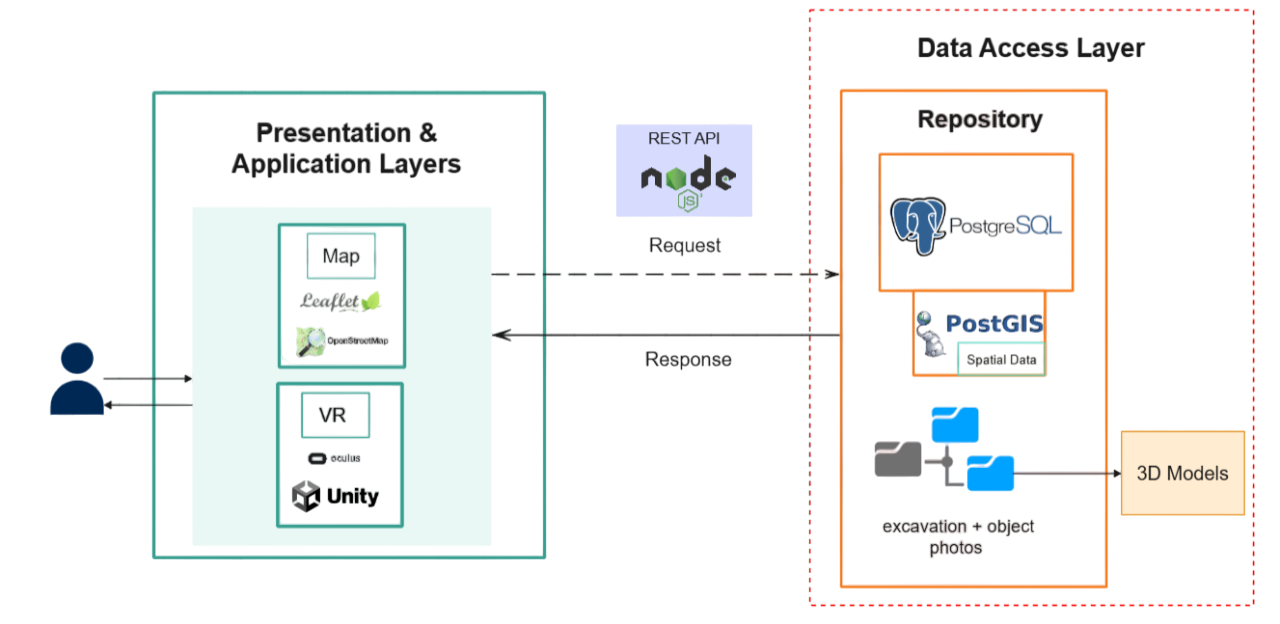
\includegraphics[width=1.0\linewidth]{system_architecture2}
% \caption{System Architecture Overview}
% \label{fig:architecture}
% \end{figure}
% \FloatBarrier

% \section{Usability Tests}
% \label{sec:usability_tests}

% The Usability Tests will be conducted both remotely and presencially throughout the implementation process, specifically the \gls{HMD} interactions will be done in person.
% Investigators from \gls{VICARTE} will participate in these tests with valuable feedback to improve the platform, while providing input on their archeology necessities. Their collaboration will contribute to a more useful, accurate, and user-friendly platform.

% \section{Previous Work}
% \label{sec:previous_work}

% During the curricular internship, a platform was developed using React\footnote{\url{https://react.dev/}} and TailwindCSS for the web layer, with C\# and ASP.NET for the application layer, and MongoDB\footnote{\url{https://www.mongodb.com/}} for data storage. Communication between these three components was handled through direct requests to the web server, which forwarded \gls{CRUD} operations and interacted with the database.  
% Additionally, the Database Systems and Cloud Computation Systems master's course provided hands-on experience in various storage methodologies and introduced different technologies and alternative solutions for data management.

% This section explains the various experiments carried out during the preparation phase.

% \subsection{Web \gls{GIS}}
% \label{sec:gis_previous} 

% To further develop expertise in \gls{GIS}, enrollment was made in the master's GeoWeb course taught by the thesis adviser, Armanda Rodrigues. During this course, was developed a Web \gls{3D} application designed to provide an interactive map for visualizing and analyzing demographic data, key infrastructure locations, and other notable European datasets. Although this project did not focus on archaeological data, it introduced and enriched the understanding of GIS concepts, map interaction, and geospatial analysis while exposing new technologies.

% The application leveraged PostGIS, a PostgreSQL extension that supports spatial operations.
% Additionally, frameworks like Leaflet were used for map rendering, visualization, and user interaction. For the base map, \gls{OSM} was integrated, offering a customizable and versatile visualization. This project serves as a preparatory stage for my thesis, specifically for the \gls{GIS} component, in which I will develop an interactive map of the Troia site.

% \section{Data Structure Proposal}
% \label{sec:data_strucutre}

% A preliminary database structure has been proposed and analysed for artefacts storage management.  
% It incorporates the key characteristics of each object to ensure structured organization and availability.

% \begin{figure}[h!]
%     \centering
%     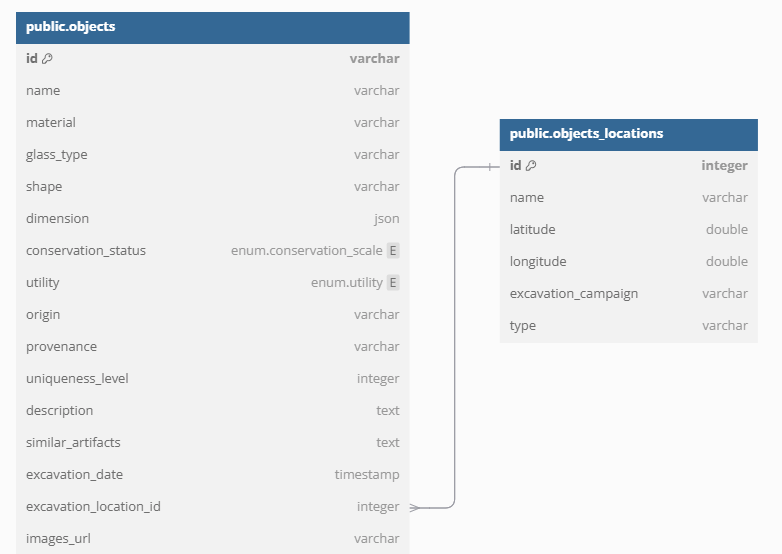
\includegraphics[width=0.7\textwidth]{data_structure}
%     \caption{Proposed Data Structure for Managing Artifacts Data.}
%     \label{fig:data_strucutre}
% \end{figure}
% \FloatBarrier

% \subsection{Photogrammetry}
% \label{sec:photogrammetry_previous} 

% During the preparation, a photogrammetric experiment was conducted by the student using the \textit{Agisoft Metashape} environment. A total of 143 images were collected during the excavation campaign by the restoration department of NOVA for analysis. 
% Based on these images, a \gls{3D} model was generated from the photogrammetric survey and subsequently imported into the \textit{Sketchfab} viewer for intuitive interaction.
% Within the grave where the deceased was buried, three open triangular areas were identified, containing the precious artefacts of the defunct, as shown in Figure~\ref{fig:model3} below.

% \begin{figure}[h!]
%     \centering
%     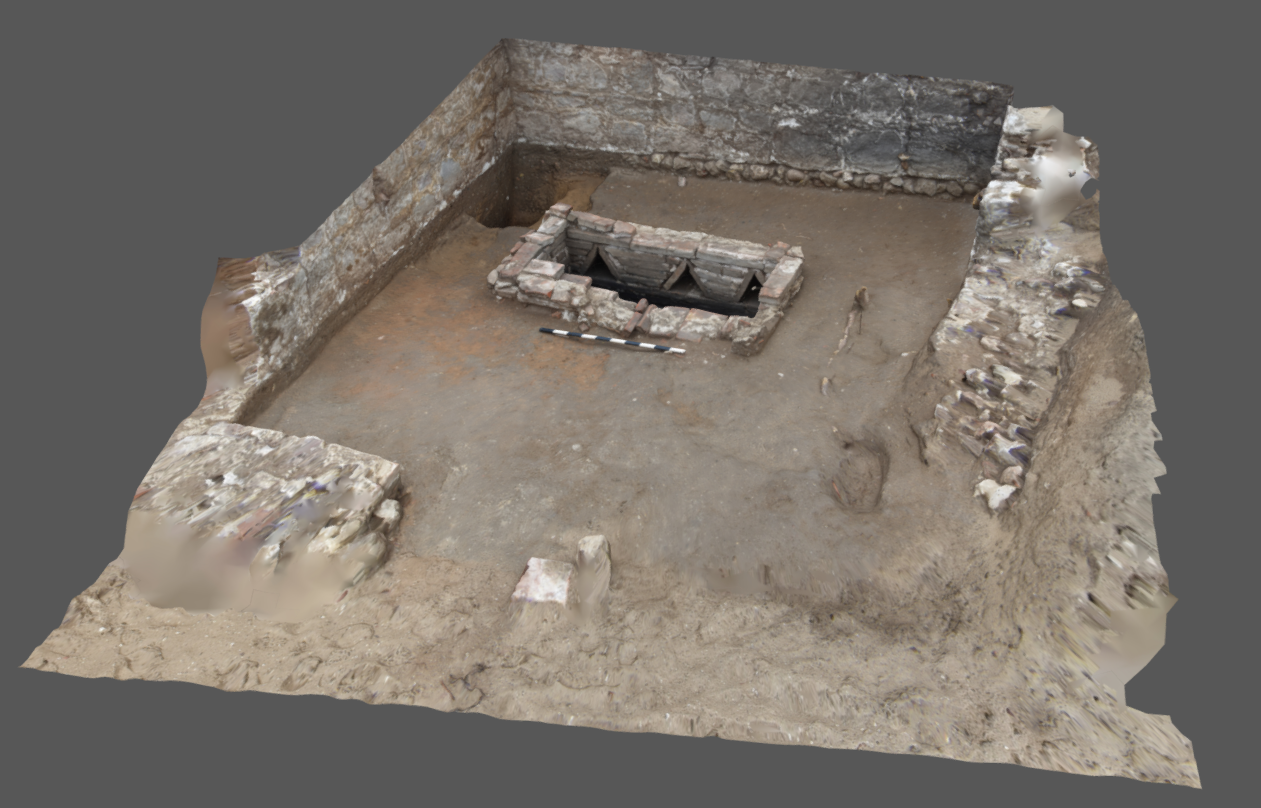
\includegraphics[width=0.7\textwidth]{model3}
%     \caption{\gls{3D} Model Imported into Sketchfab for Visualization.}
%     \label{fig:model3}
% \end{figure}
% \FloatBarrier

% \subsection{Unity}
% \label{sec:unity} 

% To reproduce the visualization of the \gls{3D} models on the map, a simulation was created in Unity, as presented in Figure \ref{fig:overlay}. The goal was to overlay the map with the \gls{3D} excavation model.
% To achieve this, the illustrated map was placed as the ground surface, with the excavation model positioned above it. The ultimate objective is to apply this approach to the artefacts found within the three triangular areas of the grave.

% This experiment simulates an intended interactive and dynamic experience, allowing users to explore the map and objects through interactive layers while using an \gls{HMD}.

% \begin{figure}[h!]
%     \centering
%     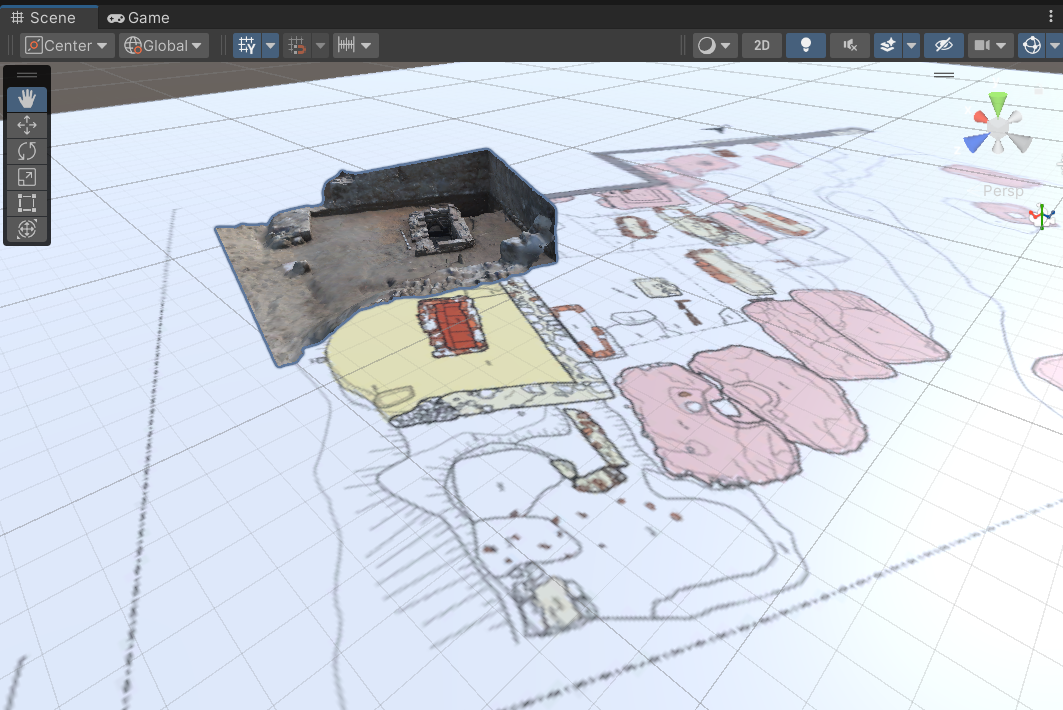
\includegraphics[width=0.7\textwidth]{overlay_test}
%     \caption{Overlay \gls{3D} Excavation Model with a Map Representation.}
%     \label{fig:overlay}
% \end{figure}
% \FloatBarrier


% \section{Work Plan}
% \label{cha:work_plan}

% This section contains the planned progress, organized into distinct tasks, each with a description. Some tasks will be developed in parallel. 
% Additionally, a Gantt chart is presented in Figure \ref{fig:gantt_chart} to illustrate the timeline for each task.

% \begin{itemize}
%     \item \textbf{Mockup Development}: This task focuses on developing a mockup that includes map visualization within a \gls{VE}, along with the associated functionalities and \gls{3D} models visualization.
%     \item \textbf{\gls{VE} Development}: This phase involves creating an immersive environment where users can navigate, and select objects, followed by the implementation of interactive functionalities with \gls{3D} models of the artefacts. These interactions include applying filters, zooming, and scaling. Initially, the development will focus on a simulation with a single object.
%     \item \textbf{\gls{GIS} Implementation}: This task comprises the creation of a map that allows user interaction with \gls{POI} represented by markers, integrating layers, and providing functionalities as outlined in Section \ref{sec:requirements}. Although the \gls{GIS} and \gls{VR} tools are developed in parallel, it may be possible to transfer from the map to the immersive environment through user interaction (e.g., clicking on a location on the map to display its \gls{3D} model), or the other way around.
%     \item \textbf{Database Creation for Repository}: In this phase, a database will be established to store significant data, including artefact and excavation metadata. The structure will initially focus on a single object, as proposed in Section \ref{sec:data_strucutre}. The database will be continuously updated over several weeks to data loading and modifications.
%     \item \textbf{System Evaluation \& Testing}: This task involves testing functionalities, usability, and performance, with participation from VICARTE investigators. Following the conclusion of the testing phase, the system evaluation process will begin with user questionnaires, leading to potential improvements based on the feedback received.  
%     \item \textbf{Documentation}: The dissertation report will be developed during the whole process.
% \end{itemize}

% % \begin{figure}[h!]
% %     \centering
% %     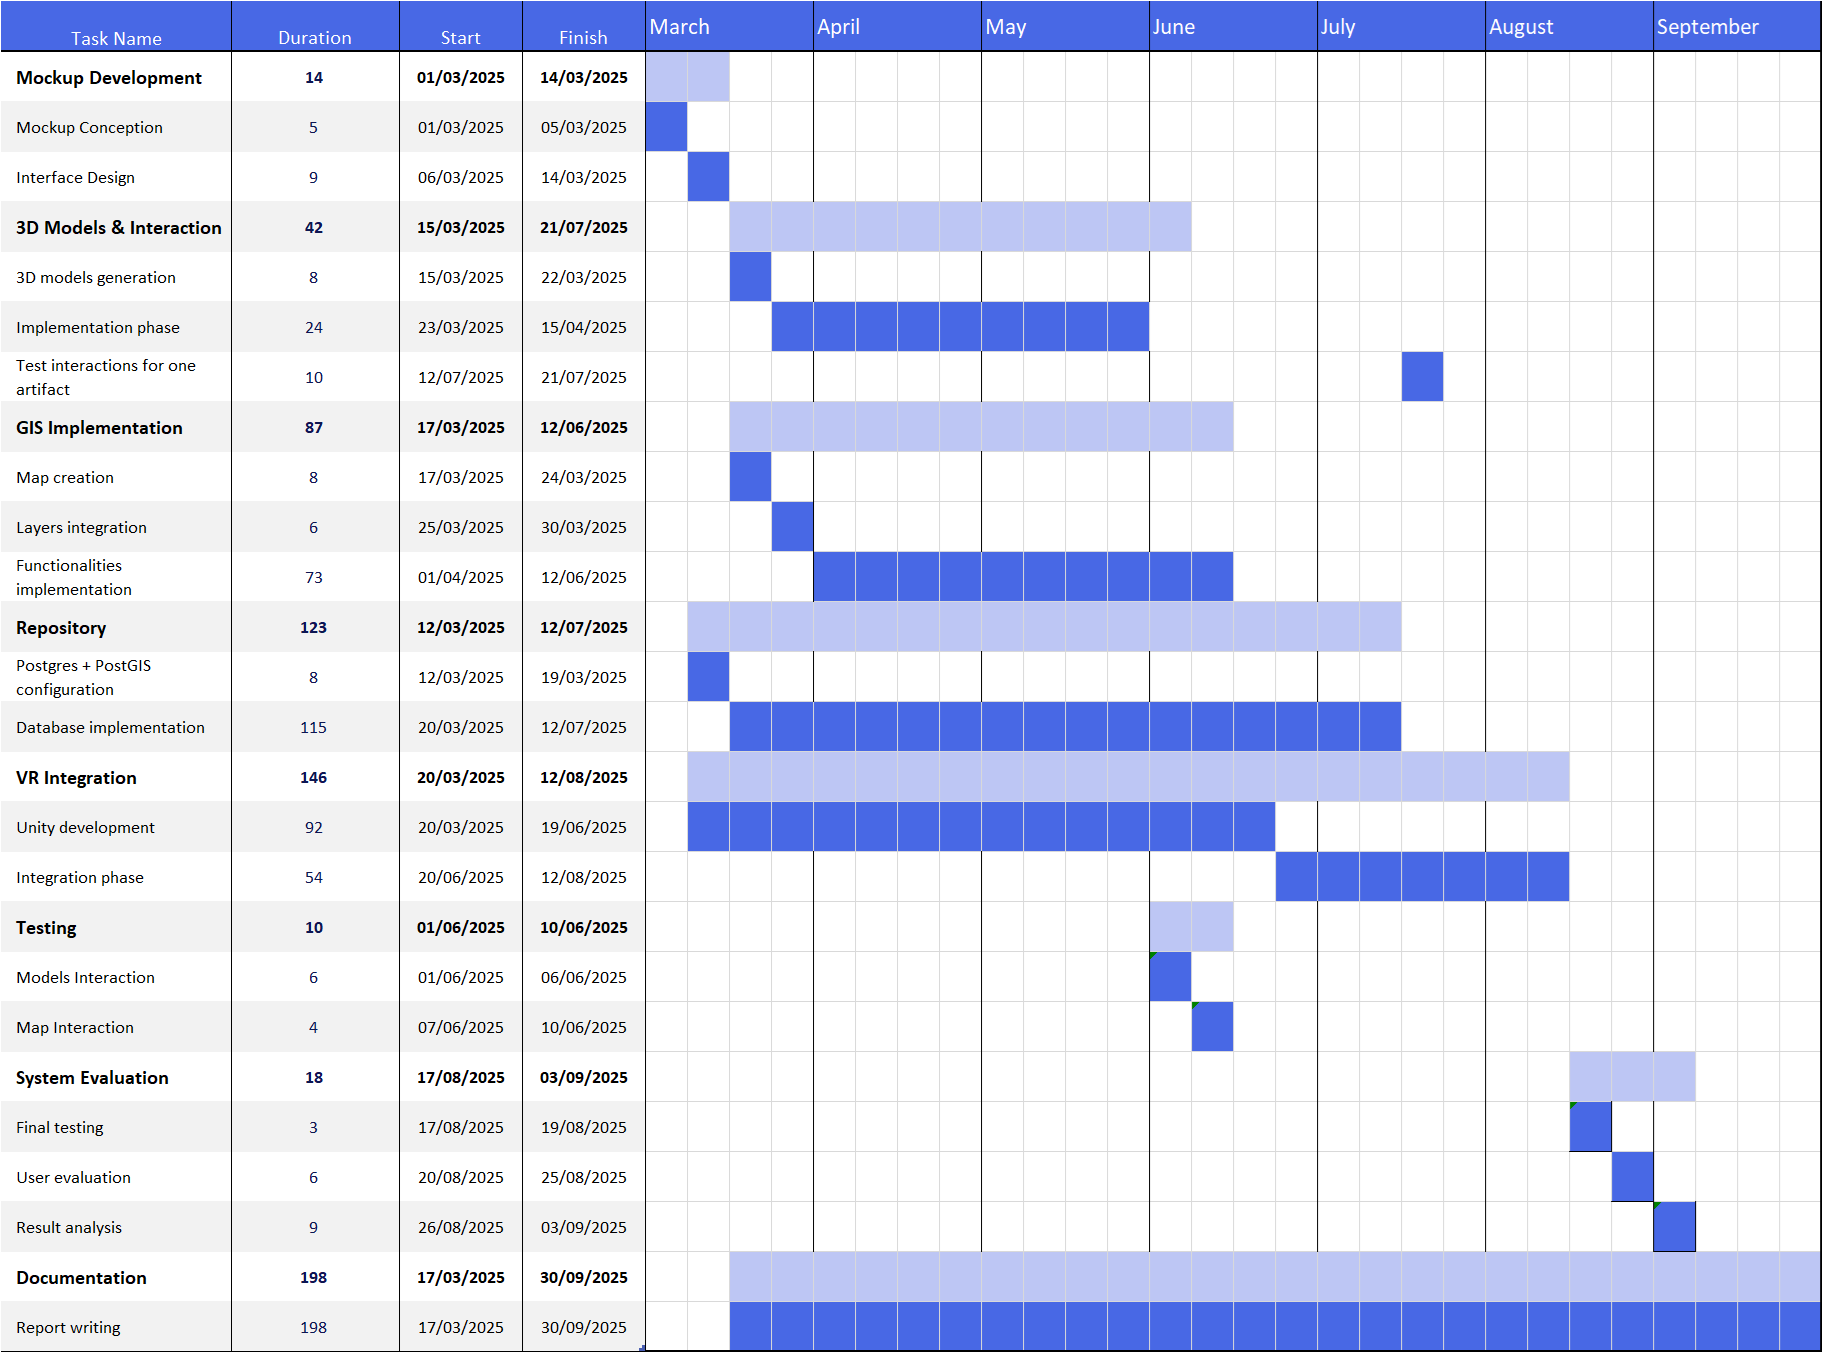
\includegraphics[width=1.0\linewidth]{Gantt_chart}
% %     \caption{Gantt Chart Representation of the Work Plan.}
% %     \label{fig:gantt_chart}
% %   \end{figure}
% %   \FloatBarrier


% %   \begin{figure}[h!]
% %     \centering
% %     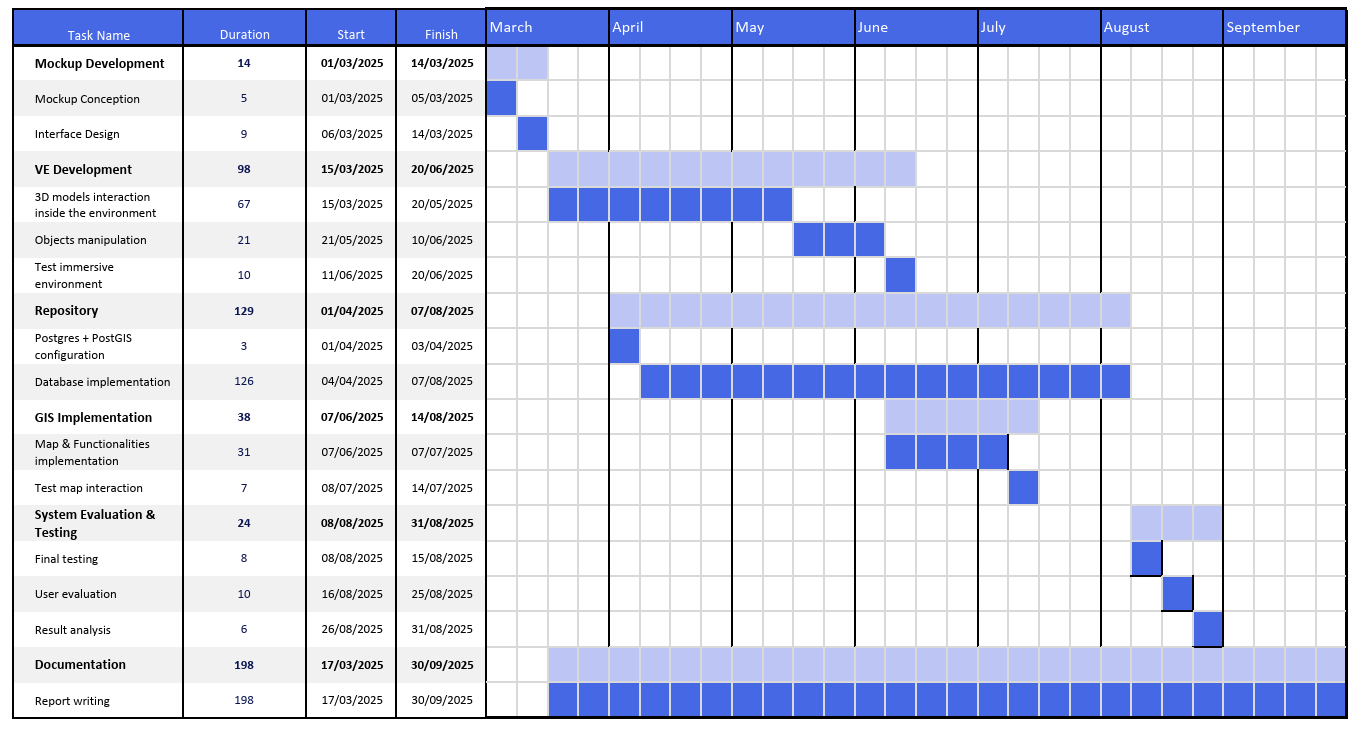
\includegraphics[width=1.0\linewidth]{gantt_chartt}
% %     \caption{Gantt Chart Representation of the Work Plan.}
% %     \label{fig:gantt_chart}
% %   \end{figure}
% %   \FloatBarrier

%   \begin{figure}[h!]
%     \centering
%     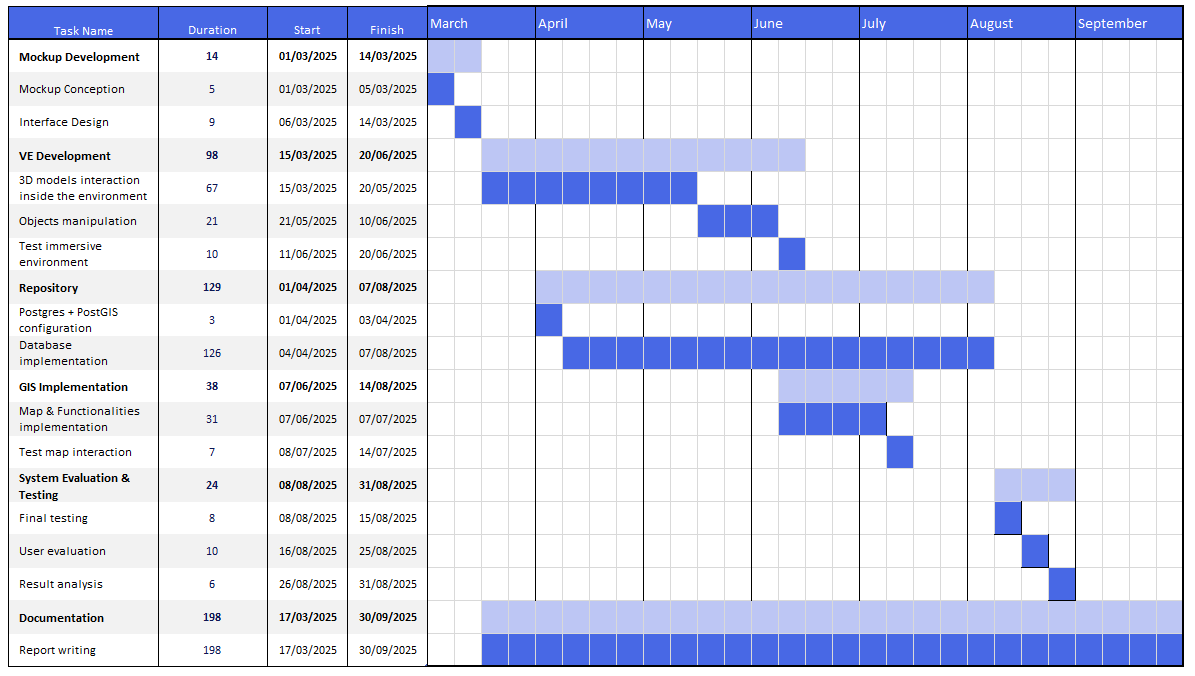
\includegraphics[width=1.0\linewidth]{gantt_chartt2}
%     \caption{Gantt Chart Representation of the Work Plan.}
%     \label{fig:gantt_chart}
%   \end{figure}
%   \FloatBarrier


